
%
\documentclass[journal, hidelinks]{IEEEtran}
%
% If IEEEtran.cls has not been installed into the LaTeX system files,
% manually specify the path to it like:
% \documentclass[journal]{../sty/IEEEtran}





% Some very useful LaTeX packages include:
% (uncomment the ones you want to load)


% *** MISC UTILITY PACKAGES ***
%
%\usepackage{ifpdf}
% Heiko Oberdiek's ifpdf.sty is very useful if you need conditional
% compilation based on whether the output is pdf or dvi.
% usage:
% \ifpdf
%   % pdf code
% \else
%   % dvi code
% \fi
% The latest version of ifpdf.sty can be obtained from:
% http://www.ctan.org/tex-archive/macros/latex/contrib/oberdiek/
% Also, note that IEEEtran.cls V1.7 and later provides a builtin
% \ifCLASSINFOpdf conditional that works the same way.
% When switching from latex to pdflatex and vice-versa, the compiler may
% have to be run twice to clear warning/error messages.






% *** CITATION PACKAGES ***
%
%\usepackage{cite}
% cite.sty was written by Donald Arseneau
% V1.6 and later of IEEEtran pre-defines the format of the cite.sty package
% \cite{} output to follow that of IEEE. Loading the cite package will
% result in citation numbers being automatically sorted and properly
% "compressed/ranged". e.g., [1], [9], [2], [7], [5], [6] without using
% cite.sty will become [1], [2], [5]--[7], [9] using cite.sty. cite.sty's
% \cite will automatically add leading space, if needed. Use cite.sty's
% noadjust option (cite.sty V3.8 and later) if you want to turn this off.
% cite.sty is already installed on most LaTeX systems. Be sure and use
% version 4.0 (2003-05-27) and later if using hyperref.sty. cite.sty does
% not currently provide for hyperlinked citations.
% The latest version can be obtained at:
% http://www.ctan.org/tex-archive/macros/latex/contrib/cite/
% The documentation is contained in the cite.sty file itself.






% *** GRAPHICS RELATED PACKAGES ***
%
\ifCLASSINFOpdf
% \usepackage[pdftex]{graphicx}
% declare the path(s) where your graphic files are
% \graphicspath{{../pdf/}{../jpeg/}}
% and their extensions so you won't have to specify these with
% every instance of \includegraphics
% \DeclareGraphicsExtensions{.pdf,.jpeg,.png}
\else
% or other class option (dvipsone, dvipdf, if not using dvips). graphicx
% will default to the driver specified in the system graphics.cfg if no
% driver is specified.
% \usepackage[dvips]{graphicx}
% declare the path(s) where your graphic files are
% \graphicspath{{../eps/}}
% and their extensions so you won't have to specify these with
% every instance of \includegraphics
% \DeclareGraphicsExtensions{.eps}
\fi
% graphicx was written by David Carlisle and Sebastian Rahtz. It is
% required if you want graphics, photos, etc. graphicx.sty is already
% installed on most LaTeX systems. The latest version and documentation can
% be obtained at: 
% http://www.ctan.org/tex-archive/macros/latex/required/graphics/
% Another good source of documentation is "Using Imported Graphics in
% LaTeX2e" by Keith Reckdahl which can be found as epslatex.ps or
% epslatex.pdf at: http://www.ctan.org/tex-archive/info/
%
% latex, and pdflatex in dvi mode, support graphics in encapsulated
% postscript (.eps) format. pdflatex in pdf mode supports graphics
% in .pdf, .jpeg, .png and .mps (metapost) formats. Users should ensure
% that all non-photo figures use a vector format (.eps, .pdf, .mps) and
% not a bitmapped formats (.jpeg, .png). IEEE frowns on bitmapped formats
% which can result in "jaggedy"/blurry rendering of lines and letters as
% well as large increases in file sizes.
%
% You can find documentation about the pdfTeX application at:
% http://www.tug.org/applications/pdftex





% *** MATH PACKAGES ***
%
%\usepackage[cmex10]{amsmath}
% A popular package from the American Mathematical Society that provides
% many useful and powerful commands for dealing with mathematics. If using
% it, be sure to load this package with the cmex10 option to ensure that
% only type 1 fonts will utilized at all point sizes. Without this option,
% it is possible that some math symbols, particularly those within
% footnotes, will be rendered in bitmap form which will result in a
% document that can not be IEEE Xplore compliant!
%
% Also, note that the amsmath package sets \interdisplaylinepenalty to 10000
% thus preventing page breaks from occurring within multiline equations. Use:
%\interdisplaylinepenalty=2500
% after loading amsmath to restore such page breaks as IEEEtran.cls normally
% does. amsmath.sty is already installed on most LaTeX systems. The latest
% version and documentation can be obtained at:
% http://www.ctan.org/tex-archive/macros/latex/required/amslatex/math/





% *** SPECIALIZED LIST PACKAGES ***
%
%\usepackage{algorithmic}
% algorithmic.sty was written by Peter Williams and Rogerio Brito.
% This package provides an algorithmic environment fo describing algorithms.
% You can use the algorithmic environment in-text or within a figure
% environment to provide for a floating algorithm. Do NOT use the algorithm
% floating environment provided by algorithm.sty (by the same authors) or
% algorithm2e.sty (by Christophe Fiorio) as IEEE does not use dedicated
% algorithm float types and packages that provide these will not provide
% correct IEEE style captions. The latest version and documentation of
% algorithmic.sty can be obtained at:
% http://www.ctan.org/tex-archive/macros/latex/contrib/algorithms/
% There is also a support site at:
% http://algorithms.berlios.de/index.html
% Also of interest may be the (relatively newer and more customizable)
% algorithmicx.sty package by Szasz Janos:
% http://www.ctan.org/tex-archive/macros/latex/contrib/algorithmicx/




% *** ALIGNMENT PACKAGES ***
%
%\usepackage{array}
% Frank Mittelbach's and David Carlisle's array.sty patches and improves
% the standard LaTeX2e array and tabular environments to provide better
% appearance and additional user controls. As the default LaTeX2e table
% generation code is lacking to the point of almost being broken with
% respect to the quality of the end results, all users are strongly
% advised to use an enhanced (at the very least that provided by array.sty)
% set of table tools. array.sty is already installed on most systems. The
% latest version and documentation can be obtained at:
% http://www.ctan.org/tex-archive/macros/latex/required/tools/


%\usepackage{mdwmath}
%\usepackage{mdwtab}
% Also highly recommended is Mark Wooding's extremely powerful MDW tools,
% especially mdwmath.sty and mdwtab.sty which are used to format equations
% and tables, respectively. The MDWtools set is already installed on most
% LaTeX systems. The lastest version and documentation is available at:
% http://www.ctan.org/tex-archive/macros/latex/contrib/mdwtools/


% IEEEtran contains the IEEEeqnarray family of commands that can be used to
% generate multiline equations as well as matrices, tables, etc., of high
% quality.


%\usepackage{eqparbox}
% Also of notable interest is Scott Pakin's eqparbox package for creating
% (automatically sized) equal width boxes - aka "natural width parboxes".
% Available at:
% http://www.ctan.org/tex-archive/macros/latex/contrib/eqparbox/





% *** SUBFIGURE PACKAGES ***
%\usepackage[tight,footnotesize]{subfigure}
% subfigure.sty was written by Steven Douglas Cochran. This package makes it
% easy to put subfigures in your figures. e.g., "Figure 1a and 1b". For IEEE
% work, it is a good idea to load it with the tight package option to reduce
% the amount of white space around the subfigures. subfigure.sty is already
% installed on most LaTeX systems. The latest version and documentation can
% be obtained at:
% http://www.ctan.org/tex-archive/obsolete/macros/latex/contrib/subfigure/
% subfigure.sty has been superceeded by subfig.sty.



%\usepackage[caption=false]{caption}
%\usepackage[font=footnotesize]{subfig}
% subfig.sty, also written by Steven Douglas Cochran, is the modern
% replacement for subfigure.sty. However, subfig.sty requires and
% automatically loads Axel Sommerfeldt's caption.sty which will override
% IEEEtran.cls handling of captions and this will result in nonIEEE style
% figure/table captions. To prevent this problem, be sure and preload
% caption.sty with its "caption=false" package option. This is will preserve
% IEEEtran.cls handing of captions. Version 1.3 (2005/06/28) and later 
% (recommended due to many improvements over 1.2) of subfig.sty supports
% the caption=false option directly:
%\usepackage[caption=false,font=footnotesize]{subfig}
%
% The latest version and documentation can be obtained at:
% http://www.ctan.org/tex-archive/macros/latex/contrib/subfig/
% The latest version and documentation of caption.sty can be obtained at:
% http://www.ctan.org/tex-archive/macros/latex/contrib/caption/




% *** FLOAT PACKAGES ***
%
%\usepackage{fixltx2e}
% fixltx2e, the successor to the earlier fix2col.sty, was written by
% Frank Mittelbach and David Carlisle. This package corrects a few problems
% in the LaTeX2e kernel, the most notable of which is that in current
% LaTeX2e releases, the ordering of single and double column floats is not
% guaranteed to be preserved. Thus, an unpatched LaTeX2e can allow a
% single column figure to be placed prior to an earlier double column
% figure. The latest version and documentation can be found at:
% http://www.ctan.org/tex-archive/macros/latex/base/



%\usepackage{stfloats}
% stfloats.sty was written by Sigitas Tolusis. This package gives LaTeX2e
% the ability to do double column floats at the bottom of the page as well
% as the top. (e.g., "\begin{figure*}[!b]" is not normally possible in
% LaTeX2e). It also provides a command:
%\fnbelowfloat
% to enable the placement of footnotes below bottom floats (the standard
% LaTeX2e kernel puts them above bottom floats). This is an invasive package
% which rewrites many portions of the LaTeX2e float routines. It may not work
% with other packages that modify the LaTeX2e float routines. The latest
% version and documentation can be obtained at:
% http://www.ctan.org/tex-archive/macros/latex/contrib/sttools/
% Documentation is contained in the stfloats.sty comments as well as in the
% presfull.pdf file. Do not use the stfloats baselinefloat ability as IEEE
% does not allow \baselineskip to stretch. Authors submitting work to the
% IEEE should note that IEEE rarely uses double column equations and
% that authors should try to avoid such use. Do not be tempted to use the
% cuted.sty or midfloat.sty packages (also by Sigitas Tolusis) as IEEE does
% not format its papers in such ways.


%\ifCLASSOPTIONcaptionsoff
%  \usepackage[nomarkers]{endfloat}
% \let\MYoriglatexcaption\caption
% \renewcommand{\caption}[2][\relax]{\MYoriglatexcaption[#2]{#2}}
%\fi
% endfloat.sty was written by James Darrell McCauley and Jeff Goldberg.
% This package may be useful when used in conjunction with IEEEtran.cls'
% captionsoff option. Some IEEE journals/societies require that submissions
% have lists of figures/tables at the end of the paper and that
% figures/tables without any captions are placed on a page by themselves at
% the end of the document. If needed, the draftcls IEEEtran class option or
% \CLASSINPUTbaselinestretch interface can be used to increase the line
% spacing as well. Be sure and use the nomarkers option of endfloat to
% prevent endfloat from "marking" where the figures would have been placed
% in the text. The two hack lines of code above are a slight modification of
% that suggested by in the endfloat docs (section 8.3.1) to ensure that
% the full captions always appear in the list of figures/tables - even if
% the user used the short optional argument of \caption[]{}.
% IEEE papers do not typically make use of \caption[]'s optional argument,
% so this should not be an issue. A similar trick can be used to disable
% captions of packages such as subfig.sty that lack options to turn off
% the subcaptions:
% For subfig.sty:
% \let\MYorigsubfloat\subfloat
% \renewcommand{\subfloat}[2][\relax]{\MYorigsubfloat[]{#2}}
% For subfigure.sty:
% \let\MYorigsubfigure\subfigure
% \renewcommand{\subfigure}[2][\relax]{\MYorigsubfigure[]{#2}}
% However, the above trick will not work if both optional arguments of
% the \subfloat/subfig command are used. Furthermore, there needs to be a
% description of each subfigure *somewhere* and endfloat does not add
% subfigure captions to its list of figures. Thus, the best approach is to
% avoid the use of subfigure captions (many IEEE journals avoid them anyway)
% and instead reference/explain all the subfigures within the main caption.
% The latest version of endfloat.sty and its documentation can obtained at:
% http://www.ctan.org/tex-archive/macros/latex/contrib/endfloat/
%
% The IEEEtran \ifCLASSOPTIONcaptionsoff conditional can also be used
% later in the document, say, to conditionally put the References on a 
% page by themselves.





% *** PDF, URL AND HYPERLINK PACKAGES ***
%
\usepackage{url}
% url.sty was written by Donald Arseneau. It provides better support for
% handling and breaking URLs. url.sty is already installed on most LaTeX
% systems. The latest version can be obtained at:
% http://www.ctan.org/tex-archive/macros/latex/contrib/misc/
% Read the url.sty source comments for usage information. Basically,
% \url{my_url_here}.





% *** Do not adjust lengths that control margins, column widths, etc. ***
% *** Do not use packages that alter fonts (such as pslatex).         ***
% There should be no need to do such things with IEEEtran.cls V1.6 and later.
% (Unless specifically asked to do so by the journal or conference you plan
% to submit to, of course. )


% correct bad hyphenation here
\hyphenation{op-tical net-works semi-conduc-tor}
\usepackage[table]{xcolor}
\usepackage{colortbl,bm}
\usepackage[backend=bibtex,style=ieee, maxbibnames=99]{biblatex}
\usepackage{multirow,graphicx}
\usepackage{multirow}
\usepackage{subfig}
\usepackage{stfloats}
\usepackage{hyperref}
\usepackage{multicol}
\usepackage[flushleft]{threeparttable}
\usepackage{mathtools}
\usepackage{csquotes}
\newcolumntype{C}{>{$}c<{$}} % math-mode version of "l" column type
\newenvironment{conditions}
{\par\vspace{\abovedisplayskip}\noindent\begin{tabular}{>{$}l<{$} @{${}={}$} l}}
{\end{tabular}\par\vspace{\belowdisplayskip}}
\addbibresource{UvicThesis.bib} 
\begin{document}
\DeclarePairedDelimiter\ceil{\lceil}{\rceil}
\DeclarePairedDelimiter\floor{\lfloor}{\rfloor}
%
% paper title
% can use linebreaks \\ within to get better formatting as desired
\title{Automated Hardware Trojan Detection in FPGAs}
%
%
% author names and IEEE memberships
% note positions of commas and nonbreaking spaces ( ~ ) LaTeX will not break
% a structure at a ~ so this keeps an author's name from being broken across
% two lines.
% use \thanks{} to gain access to the first footnote area
% a separate \thanks must be used for each paragraph as LaTeX2e's \thanks
% was not built to handle multiple paragraphs
%

\author{Nicholas~Houghton,~\IEEEmembership{Member,~IEEE,}
	Samer~Moein,~\IEEEmembership{Member,~IEEE,}
	and~Fayez~Gebali,~\IEEEmembership{Life~Senior Member,~IEEE}% <-this % stops a space
	\thanks{N.~Houghton, S.~Moein, and F.~Gebali are with the Department
		of Electrical and Computer Engineering, University of Victoria, Victoria, Canada.}
	\thanks{Manuscript received November 28, 2016; revised November 30, 2016.}}

% note the % following the last \IEEEmembership and also \thanks - 
% these prevent an unwanted space from occurring between the last author name
% and the end of the author line. i.e., if you had this:
% 
% \author{....lastname \thanks{...} \thanks{...} }
%                     ^------------^------------^----Do not want these spaces!
%
% a space would be appended to the last name and could cause every name on that
% line to be shifted left slightly. This is one of those "LaTeX things". For
% instance, "\textbf{A} \textbf{B}" will typeset as "A B" not "AB". To get
% "AB" then you have to do: "\textbf{A}\textbf{B}"
% \thanks is no different in this regard, so shield the last } of each \thanks
% that ends a line with a % and do not let a space in before the next \thanks.
% Spaces after \IEEEmembership other than the last one are OK (and needed) as
% you are supposed to have spaces between the names. For what it is worth,
% this is a minor point as most people would not even notice if the said evil
% space somehow managed to creep in.



% The paper headers
\markboth{Journal of \LaTeX\ Class Files,~Vol.~6, No.~1, January~2007}%
{Shell \MakeLowercase{\textit{et al.}}: Bare Demo of IEEEtran.cls for Journals}
% The only time the second header will appear is for the odd numbered pages
% after the title page when using the twoside option.
% 
% *** Note that you probably will NOT want to include the author's ***
% *** name in the headers of peer review papers.                   ***
% You can use \ifCLASSOPTIONpeerreview for conditional compilation here if
% you desire.




% If you want to put a publisher's ID mark on the page you can do it like
% this:
%\IEEEpubid{0000--0000/00\$00.00~\copyright~2007 IEEE}
% Remember, if you use this you must call \IEEEpubidadjcol in the second
% column for its text to clear the IEEEpubid mark.



% use for special paper notices
%\IEEEspecialpapernotice{(Invited Paper)}




% make the title area
\maketitle


\begin{abstract}
	%\boldmath
	Embedded Systems have become ubiquitous in modern life; we are just as affected by their vulnerabilities as they are.
	Ensuring that the processors that control them are secure is paramount to the safety of commercial, transportation and military infrastructure.
	The market for integrated circuits is steadily being consumed by a reconfigurable type of processor known as a Field-Programmable Gate-Array (FPGA).
	The very features that make this type of device so successful also make them susceptible to attack.
	FPGAs are reconfigured by software; this makes it easy for attackers to make modification.
	Such modifications are known as hardware trojans.
	There have been many techniques and strategies to ensure that these devices are free from trojans but few have taken advantage of the central feature of these devices.
	The configuration Bitstream is the binary file which programs these devices.
	By extracting and analyzing it, a much more accurate and efficient means of detecting trojans can be achieved.
	This discussion presents a new methodology for exploiting the power of the configuration Bitstream to detect and described hardware trojans.
	A software application is developed that automates this methodology for \textit{Xilinx} FPGAs.
\end{abstract}
% IEEEtran.cls defaults to using nonbold math in the Abstract.
% This preserves the distinction between vectors and scalars. However,
% if the journal you are submitting to favors bold math in the abstract,
% then you can use LaTeX's standard command \boldmath at the very start
% of the abstract to achieve this. Many IEEE journals frown on math
% in the abstract anyway.

% Note that keywords are not normally used for peerreview papers.
%\begin{IEEEkeywords}
%	Hardware trojans, chip life cycle, hardware trojan taxonomy, hardware trojan attributes. ... Put your list
%\end{IEEEkeywords}






% For peer review papers, you can put extra information on the cover
% page as needed:
% \ifCLASSOPTIONpeerreview
% \begin{center} \bfseries EDICS Category: 3-BBND \end{center}
% \fi
%
% For peerreview papers, this IEEEtran command inserts a page break and
% creates the second title. It will be ignored for other modes.
\IEEEpeerreviewmaketitle



\section{Introduction}
% The very first letter is a 2 line initial drop letter followed
% by the rest of the first word in caps.
% 
% form to use if the first word consists of a single letter:
% \IEEEPARstart{A}{demo} file is ....
% 
% form to use if you need the single drop letter followed by
% normal text (unknown if ever used by IEEE):
% \IEEEPARstart{A}{}demo file is ....
% 
% Some journals put the first two words in caps:
% \IEEEPARstart{T}{his demo} file is ....
% 
% Here we have the typical use of a "T" for an initial drop letter
% and "HIS" in caps to complete the first word.
\IEEEPARstart{I}{n} recent years a new incarnation of electronic danger has emerged; in hardware.
In this new arena of attack and defend those who seek to defend are far behind.
Integrated Circuit (IC) designs for Field Programmable Gate-Arrays (FPGA) are made using Hardware Description Language (HDL).
The design is then converted to a binary file called a configuration Bitstream which is then downloaded onto the device; this process is known as synthesizing the design.
There have been many attempts to develop mechanisms and techniques to determine whether a malicious user has tampered with the design via test vectoring or side-channel analysis.
As of yet there has been little effort to directly analyze the configuration Bitstream.
%The majority of work focused on FPGA trojans has employed either a means of reverse engineering, functional testing or 'side-channel' analysis.


%%%%%%% Recent Work Start %%%%%%%%%%%
In 2013 researchers at Cairo University proposed a method of insulating externally sourced Intelectual Property (IP) with Cyclic Redundancy Check (CRC) defense modules~\cite{crcDetection}.
According to the authors their method is capable of detecting leaked information with a 99.95\% accuracy.
It was designed specifically for detecting trojans that leak information; trojans which exhibit other behaviors can not be detected.
In addition the authors report considerable detriment to power consumption and performance.

Researchers at the Technological Educational Institute of Western Greece and Industrial Systems Institute/RC Athena jointly~\cite{ringOscillatorMethod} proposed a method of using Ring Oscillators (RO) as a mechanism for detecting hardware trojans.
%A RO is a circuit composed of inverters formed into a loop.
%Electric current looping through the RO does so at an inherent frequency.
By configuring the circuit paths of the user's design into a RO it is possible to create a 'signature'.
This signature is an expected frequency emitted from the desired design. 
The authors claim that modifications to the design will alter the frequency emitted by its circular configuration.
The experimental results showed that modifications did in-fact alter the frequency enough to reliably detect modifications.
This method can reliably detect hardware trojans but is incapable of providing any details regarding its effect.
Further, the stipulation that the desired design must be such that it forms an oscillating ring is impractical.
It is impossible to guarantee that all real-world designs can form an RO whilst maintaining desired functionality and performance.

Researchers from Iowa State University~\cite{multiFacetedApproach} proposed a multi-faceted approach to trojan detection in FPGAs.
Their method composed of three approaches:
\begin{itemize}
	\item Functional Testing: A means of feeding test vectors and comparing the output to expected results.
	\item Power Analysis: Using an oscilloscope, the difference in power consumption between the desired design and the modified devices performing the same operations were recorded. Differences were used to discern the presence of a trojan.
	\item Bitfile Analysis: The authors attempted to employ a binary file analysis library named \textit{deBit}~\cite{bitStreamToNetlist} to reverse engineer a netlist from the Bitstream.
\end{itemize}
The functional testing method attempted provided reasonable results. 
Test vectors used showed unexpected behavior; this provided only the information that a trojan was present.
The power analysis method again provided results of moderate quality.
With careful placement of the oscilloscope probes the authors were able to infer the physical location on the device where modifications occurred.
This provided no information however as to the relation between the modifications and the design.
Finally, the authors were able to only partially convert the Bitstream to its netlist description.
Only descriptions of the primary logic circuit elements were achieved.
This could be used to discern some information regarding modifications discovered but is far from creating a complete description of a trojan.
%%%%%%% Recent Work End %%%%%%%%%%%


A new method of extracting and analyzing the configuration Bitstream to determine the presence of hardware trojans has been developed and is presented in this work.
This method is able to meaningfully read the long binary file which configures an FPGA and extract modifications.
Any discovered changes are located on the device using a technique referred to as 'Component Mapping'.
Further, these changes are then mapped to the user's original design.
Knowing which components of the device have been modified, and the instances of the synthesized design allows for a powerful description to be built.
A software tool known as the FPGA Trojan Detector, which implements this new method has been built using Java and an open-source application programming interface (API) known as RapidSmith. 
It is able to automatically detect and analyze trojans in \textit{Xilinx} FPGAs.
Once analyzed, a meaningful description is provided using the trojan taxonomy presented in~\cite{samerAttribute}.

The contributions of this paper are:
\begin{enumerate}
	\item A new method mapping configuration Bitstream words to device components named 'Component Mapping'.
	\item A systematic process of detecting and analyzing hardware trojans in FPGAs
	\item A software tool which automates these new methods.
\end{enumerate}

The remainder of this paper is organized as follows.
Section~\ref{sec:background} provides some useful background on the trojan taxonomy used by the new method, as well as the architecture of FPGAs.
Section~\ref{sec:methodolgy} describes the overall process of the new trojan detection technique.
Section~\ref{sec:trojanAttributes} presents how the analysis results of Section~\ref{sec:methodolgy} are used to generate a comprehensive description of a discovered trojan.
Section~\ref{sec:implementation} presents the software tool which demonstrates the efficacy of the new methodology.
Section~\ref{sec:results} presents three case studies using benchmark designs containing trojans.
Finally, Section~\ref{sec:conclusion} provides some concluding remarks.

%%%%%%%%%%%%%%%%%%%%%%%%%%%%%%%%%%%%%%%%%%%%%%%%%%%%%%%%%%%%%%%%%%%%
\section{Background} \label{sec:background}
\subsection{Hardware Trojan Taxonomy} \label{sec:taxonomy}
The evaluation of hardware trojans requires a comprehensive means of their description.
Several hardware trojan taxonomies have been proposed~\cite{taxonomy1, taxonomy2, taxonomy3, taxonomy4}.
An additional taxonomy was proposed in~\cite{samerAttribute} which considers all attributes a hardware trojan may posses.
This taxonomy is the most comprehensive and was selected as the means of description for this work.
It is comprised of four levels of description as shown in Fig.~\ref{fig:trojan_life_cycle}.
There are eight categories comprised of a total of thirty-three attributes as shown in Fig.~\ref{fig:HW_trojan}.

%%%%%%%%%%%%%%%%%%%%%%%


\begin{figure}[h]
	\centering
	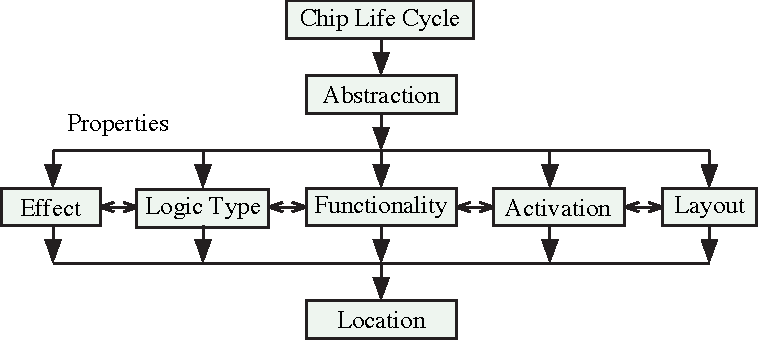
\includegraphics[width=1\linewidth]{Figures/trojan_life_cyclePDF}
	\caption{Hardware trojan life-cycle levels \cite{samerAttribute}.}
	\label{fig:trojan_life_cycle}
\end{figure}
\begin{figure*}
	\centering
	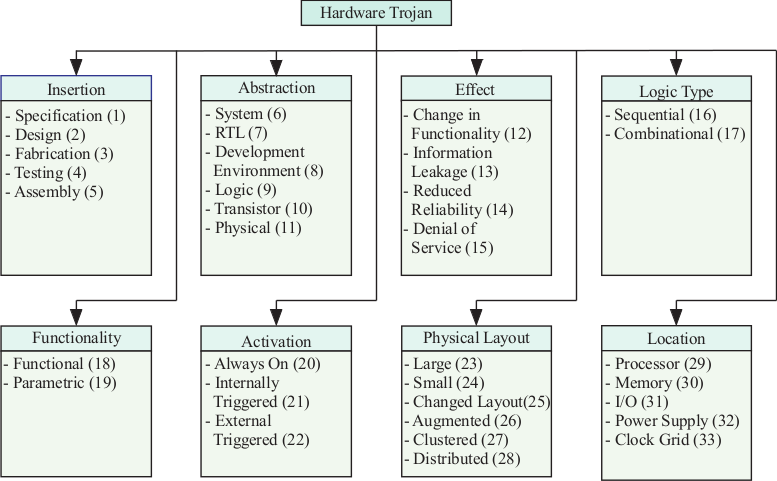
\includegraphics[width=0.775\linewidth]{Figures/HW_trojan}
	\caption{The hardware trojan attribute taxonomy \cite{samerAttribute}.}
	\label{fig:HW_trojan}
\end{figure*}

%%%%%%%%%%%%%%%%%%%%%%%%%
\begin{enumerate}
	\item The \textbf{insertion} (chip life-cycle) level comprises the attributes pertaining to the IC production stages.
	\item The \textbf{abstraction} level corresponds to where in the IC abstraction the trojan is introduced.
	\item The \textbf{properties} level comprises the behavior and physical characteristics of the trojan.
	It contains the taxonomy categories \textit{effect}, \textit{logic type}, \textit{functionality}, \textit{activation} and \textit{layout}.
	\item The \textbf{location} level corresponds to the location of the trojan in the IC.
\end{enumerate}

The properties level has the following categories.
\begin{itemize}
	\item The \textbf{effect} category describes the disruption or effect a trojan has on the system.
	\item The \textbf{logic type} category describes the circuit logic that triggers the trojan, either combinational logic or sequential.
	\item The \textbf{functionality} category differentiates between trojans which are functional or parametric.
	\item The \textbf{activation} category differentiates between trojans which are always on or are triggered.
	\item The \textbf{layout} category is based on the physical characteristics of the trojan.
\end{itemize}
The relationships between the trojan attributes shown in Fig.~\ref{fig:HW_trojan} can be described using a matrix $\mathbf{R}$~\cite{samerAttribute}.
Entry $r(i,j)$ in $\mathbf{R}$ indicates whether or not attribute $i$ can lead to attribute $j$.
For example, $r(2,3) = 1$ indicates that design (attribute 2) can lead to fabrication (attribute 3).
This implies that if an IC can be compromised during the design phase (attribute 2), it may influence the fabrication phase (attribute 3).

The matrix $\mathbf{R}$ is divided into sub matrices as follows
\[
\newcommand\scalemath[2]{\scalebox{#1}{\mbox{\ensuremath{\displaystyle #2}}}}
\mathbf{R} =\left[
\scalemath{1.1}{
	\begin{array}{l*{3}{c}}
	\mathbf{R_1} ~ & ~ \mathbf{R_{12}} ~ & ~ 0 ~  &  ~ 0   \\
	0         & \mathbf{R_2}      &\mathbf{R_{23}}       & ~ 0 \\
	0          & 0           & \mathbf{R_3}          & ~ \mathbf{R_{34}} \\
	0          & 0           & 0                & ~ \mathbf{R_4} \\
	\end{array}
}
\right]
\label{R}
\]
where $\mathbf{R_1}$, $\mathbf{R_2}$, $\mathbf{R_3}$ and $\mathbf{R_4}$ indicate the attribute relationships within a category.
For example, $\mathbf{R_1}$ is given by
\[
\newcommand\scalemath[2]{\scalebox{#1}{\mbox{\ensuremath{\displaystyle #2}}}}
\mathbf{R_1} =\left[
\scalemath{1.0}{
	\begin{array}{l|*{11}{c}}
	A & 1$~$ & 2$~$  & 3$~$ & 4$~$& 5$~$\\ \hline
	1 & 0 & 1 & 0 & 0 & 0  \\
	2 & 0 & 0 & 1 & 0 & 0  \\
	3 & 0 & 0 & 0 & 1 & 0  \\
	4 & 0 & 0 & 0 & 0 & 1  \\
	5 & 0 & 0 & 0 & 0 & 0  \\
	\end{array}
}
\right ]
\label{R1}
\]
Submatrix $\mathbf{R_{12}}$ relates the attributes of the insertion category to the attributes of the abstraction category.
An example of this submatrix is
\[
\newcommand\scalemath[2]{\scalebox{#1}{\mbox{\ensuremath{\displaystyle #2}}}}
\mathbf{R_{12}} =\left[
\scalemath{1.0}{
	\begin{array}{l|*{11}{c}}
	A & 6$~$  & 7$~$ & 8$~$ & 9$~$ & 10  & 11\\ \hline
	1  & 1 & 0 & 0 & 0 & 0 & 0 \\
	2  & 0 & 1 & 0 & 0 & 0 & 0 \\
	3  & 0 & 0 & 0 & 0 & 0 & 1 \\
	4  & 1 & 0 & 0 & 1 & 0 & 0 \\
	5  & 1 & 0 & 0 & 0 & 0 & 0 \\
	\end{array}
}
\right ]
\label{R12}
\]

%%%%%%%%%%%%%%%%%%%%%%%%%%%%%%%%
\subsection{Field Programmable Gate-Array Organization}
An Integrated Circuit (IC) belongs to one of two categories.
An Application Specific Integrated Circuit (ASIC) or a Field Programmable Gate-Array (FPGA).
An ASIC is manufactured once and is immutable; its hardware is permanently printed into its silicon.
FPGA users create designs using a programming language referred to as a Hardware Description Language (HDL).
The design is then compiled and synthesized into the Bitstream which is then downloaded or "configured" onto the device.

FPGAs are reconfigurable because they are comprised of an array of Programmable Logic Devices (PLD).
A PLD is a component whose functionality is dependent on a set of configuration options; in other words, a user can define how it behaves.
Each PLD receives configuration instructions from the user that defines its functionality; these instructions are in the form of a binary message.
The set of messages sent to all of the PLDs in the device from the user is referred to as the configuration Bitstream.

In \textit{Xilinx} terminology a PLD is referred to as a tile. 
A single FPGA can contain hundreds, or even thousands of tiles; a device is usually made up of over a hundred different types of tile.
Different types are used for different functions, such as Input-Output (IO), Logic, Memory and so on.
\begin{figure}[h]
	\centering
	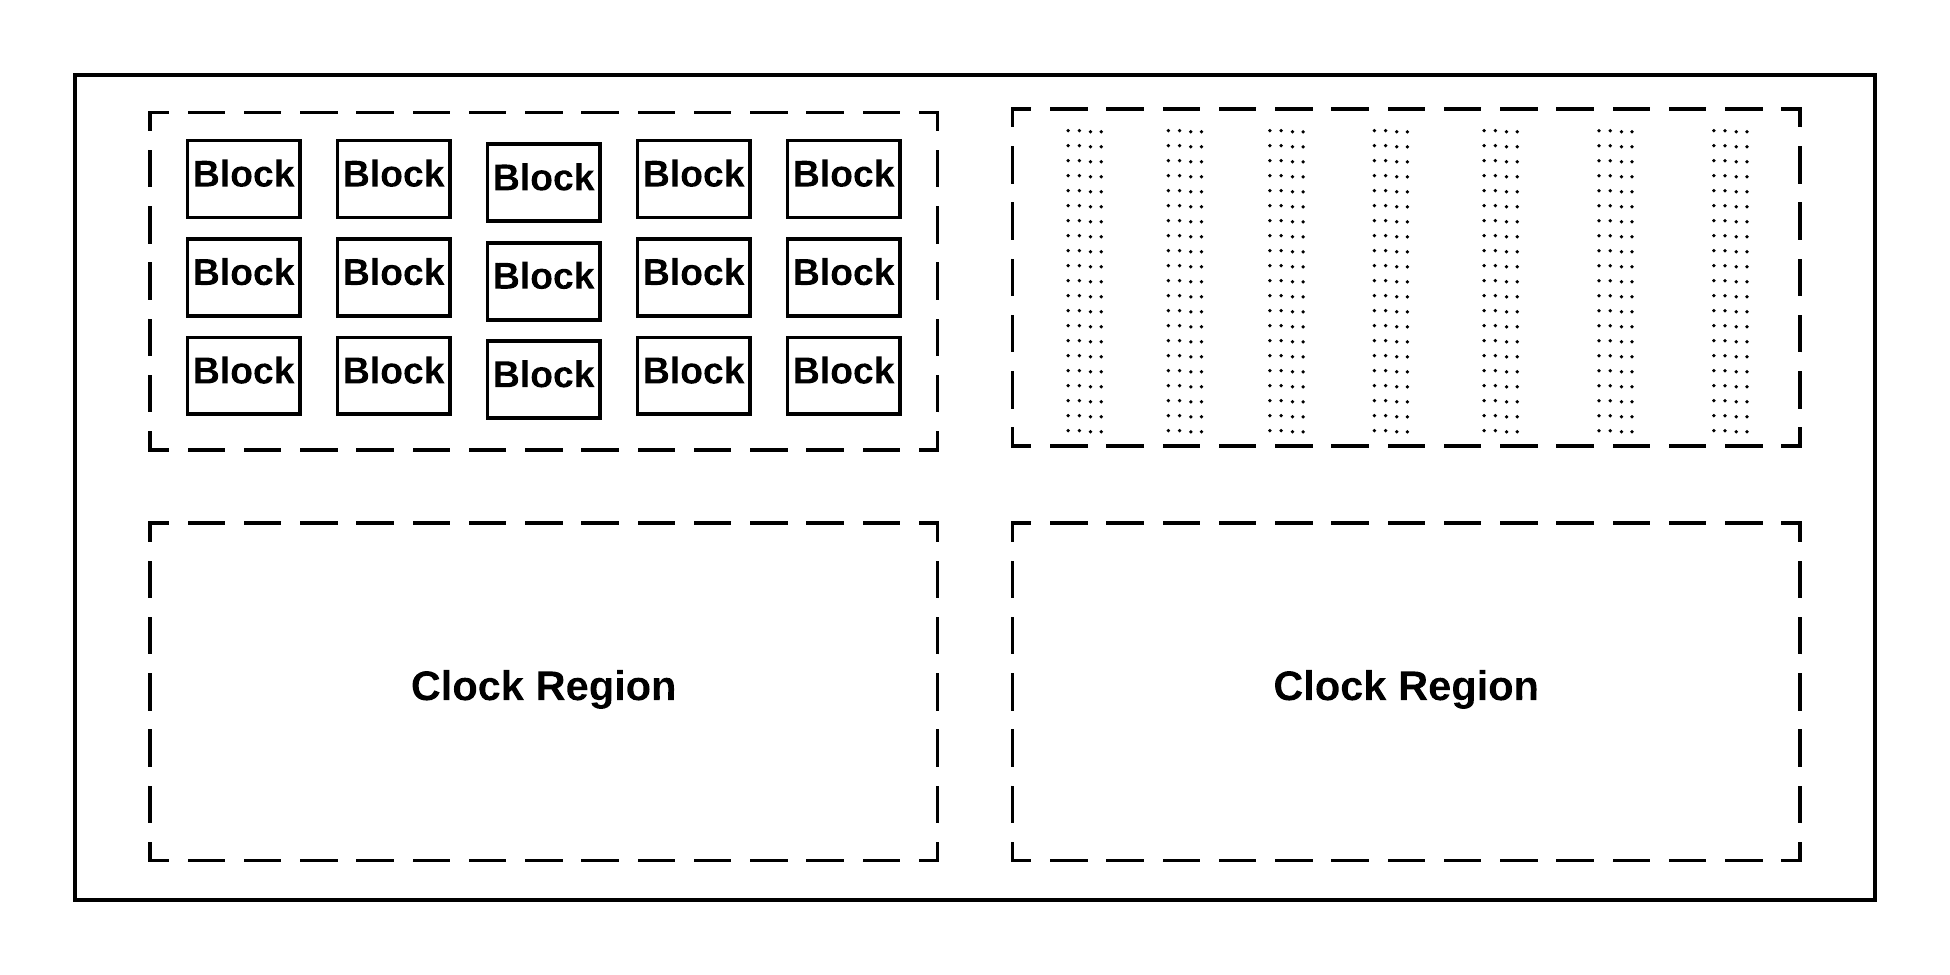
\includegraphics[width=1\linewidth]{Figures/FPGA}
	\caption[Rudimentary Layout of a Virtex FPGA]{Rudimentary Layout of a Virtex FPGA}
	\label{fig:FPGA}
\end{figure}
A \textit{Xilinx} device is organized into a matrix of blocks referred to as the 'gate-array' as shown in Fig.~\ref{fig:FPGA}~\cite{xilnxDevManual}.
A block is not a physical device but a conceptual grouping of tiles.
A block will consist of one or multiple tiles depending on its type and they are arranged into columns by type.
Columns are separated into regions shown by the dashed lines in Fig.~\ref{fig:FPGA}.
These regions each use a separate clock mechanism and are referred to as 'Clock Regions'.

%%%%%%%%%%%%%%%%%%%%%%%%%%%%%%%%%%%%%%%%%%%%%%%%%%
\section{Proposed Trojan Detection} \label{sec:methodolgy}
%%% I couldn't get this table to sit in the right place unless I put it all the way up here %%%
\begin{table*}[b!]
	\centering
	\caption{Bitstream Frame Address Structure}
	\label{tbl:frameAddress}
	\resizebox{\textwidth}{!}{
		\begin{tabular}{|c|c|c|c|c|c|c|c|c|c|c|c|c|c|c|c|c|c|c|c|c|c|c|c|c|c|c|c|c|c|c|c|}
			\hline
			\multicolumn{8}{|c|}{Unused} & \multicolumn{3}{c|}{BA} & T & \multicolumn{5}{c|}{Row Address} & \multicolumn{8}{c|}{Major Address} & \multicolumn{7}{c|}{Minor Address} \\ \hline
			31 & 30 & 29 & 28 & 27 & 26 & 25 & 24 & 23 & 22 & 21 & 20 & 19 & 18 & 17 & 16 & 15 & 14 & 13 & 12 & 11 & 10 & 9 & 8 & 7 & 6 & 5 & 4 & 3 & 2 & 1 & 0 \\ \hline
			0 & 0 & 0 & 0 & 0 & x & x & x & x & x & x & x & x & x & x & x & x & x & x & x & x & x & x & 0 & 0 & 0 & 0 & 0 & 0 & 0 & 0 & 0 \\ \hline
		\end{tabular}		
	}
\end{table*}
\subsection{Overview}
Fig.~\ref{fig:Concept} provides a visual representation of the use-case assumed for the purposes of this work. 
With the exception of the fabrication process, all stages of production of an FPGA implementation are assumed to have been done "in-house". 
Any trojan discovered is inserted in the fabrication phase; all other stages are trusted.  
The method of automated trojan detection described in this work would take place in the 'testing' phase of the life-cycle. 
\begin{figure}[h]
	\centering
	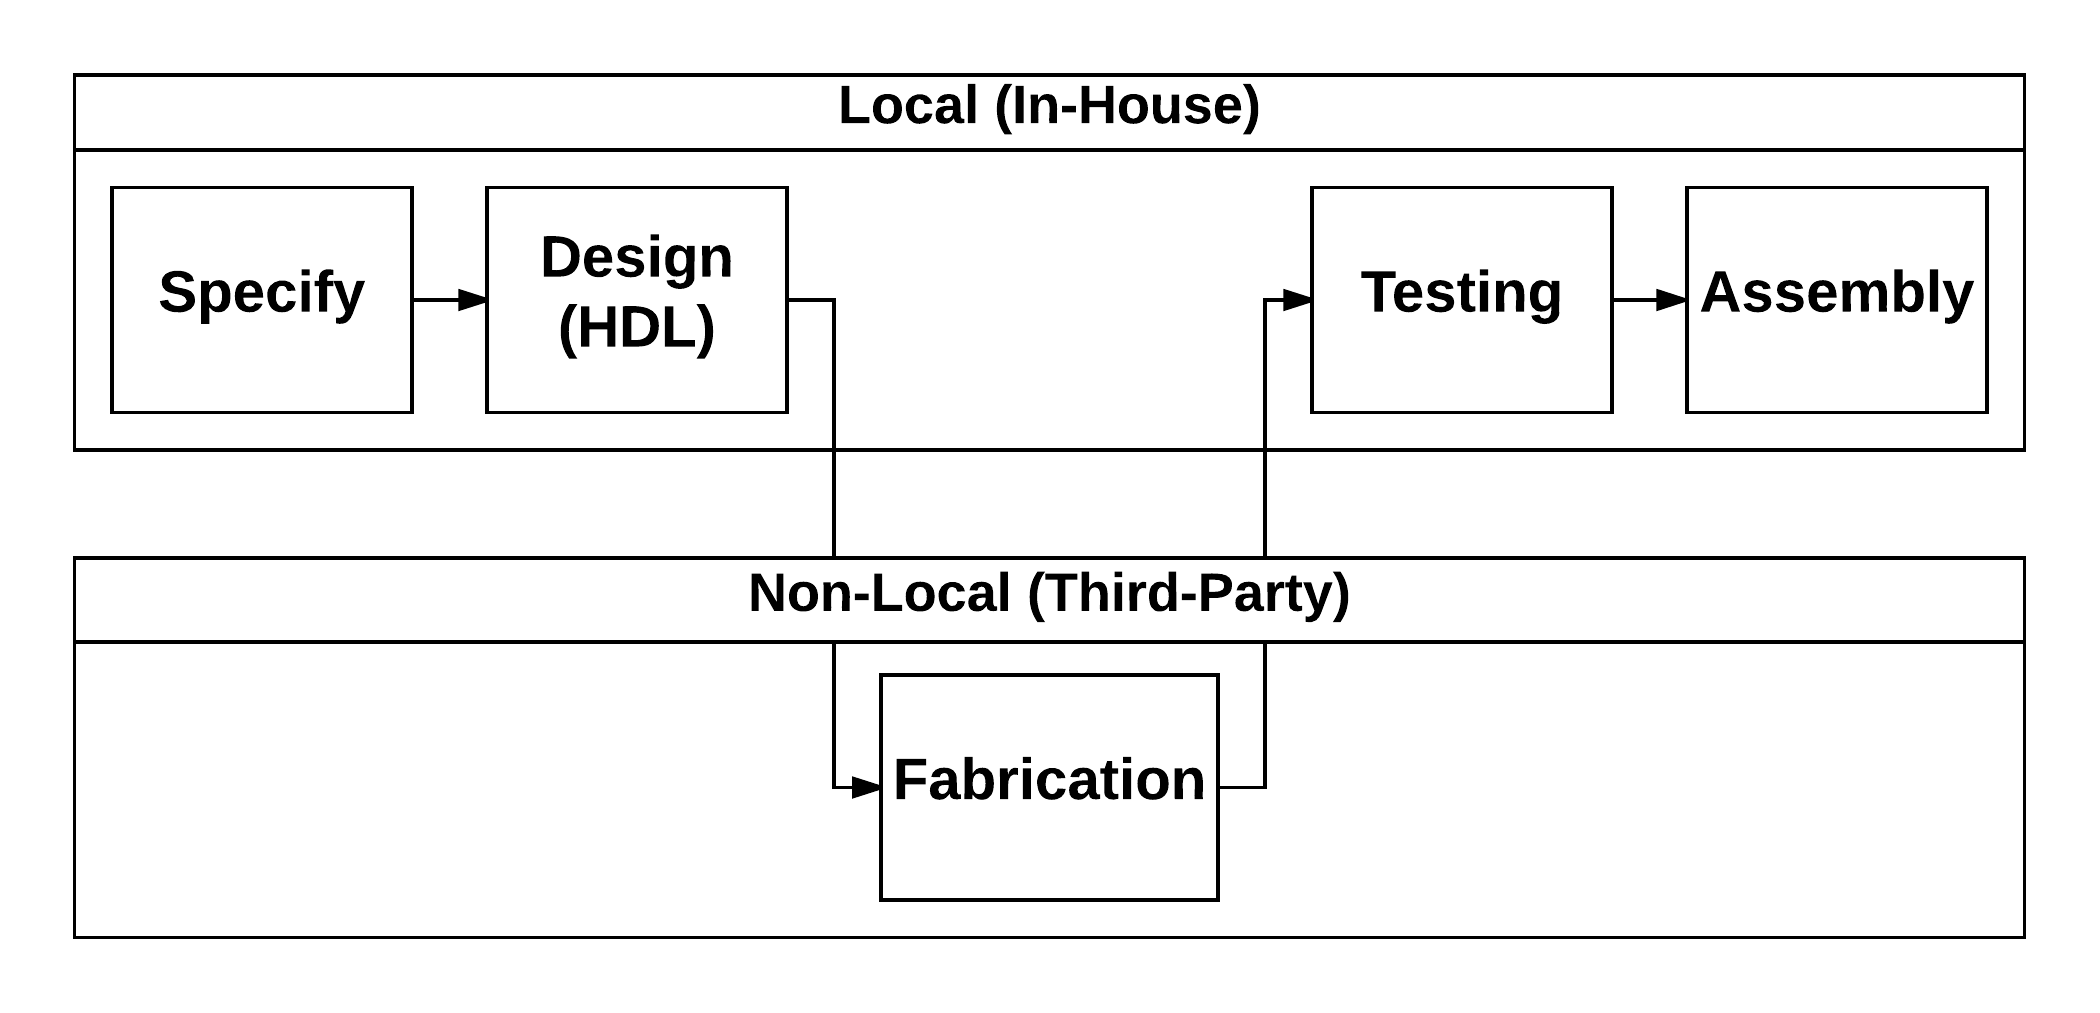
\includegraphics[width=1\linewidth]{Figures/Concept}
	\caption[FPGA Life-Cycle]{FPGA Life-Cycle}
	\label{fig:Concept}
\end{figure}
Fig.~\ref{fig:methodologyOverview} shows an overview of the trojan detection methodology.
As mentioned, FPGA designs are written in HDL.
\textit{Xilinx} provides a series of User-Interface (UI) and command line tools to process the HDL known as the 'tool-chain'.
The tool chain generates a series of files that are used for a variety of purposes as shown in the 'Resultant Files' box in Fig.~\ref{fig:methodologyOverview}.
This includes but is not limited to:
\begin{itemize}
	\item Bit: the configuration Bitstream
	\item XDL: \textit{Xilinx} Design Language
	\item NGC: a non-human readable semantic description of the design known as a netlist
	\item RDB: the readback data text file
	\item MSD: a mask file used to hide unwanted data during the a readback procedure
	\item log: a log file which collects compiler output.
\end{itemize}
The majority of these files are used for specific purposes that do not pertain to the new hardware trojan detection method.
The netlist (.ngc) file, however, contains a thorough description of the user's design and how it relates to the device.
It can be converted into a human-readable version known as a \textit{Xilinx} Design Language (XDL) file which will be used to relate any discovered modifications to the user's design.
The Bit file is the binary representation of the design implementation.
This file holds the Bitstream or 'configuration' Bitstream and is the final form that is loaded into the FPGA.
\begin{figure}
	\centering
	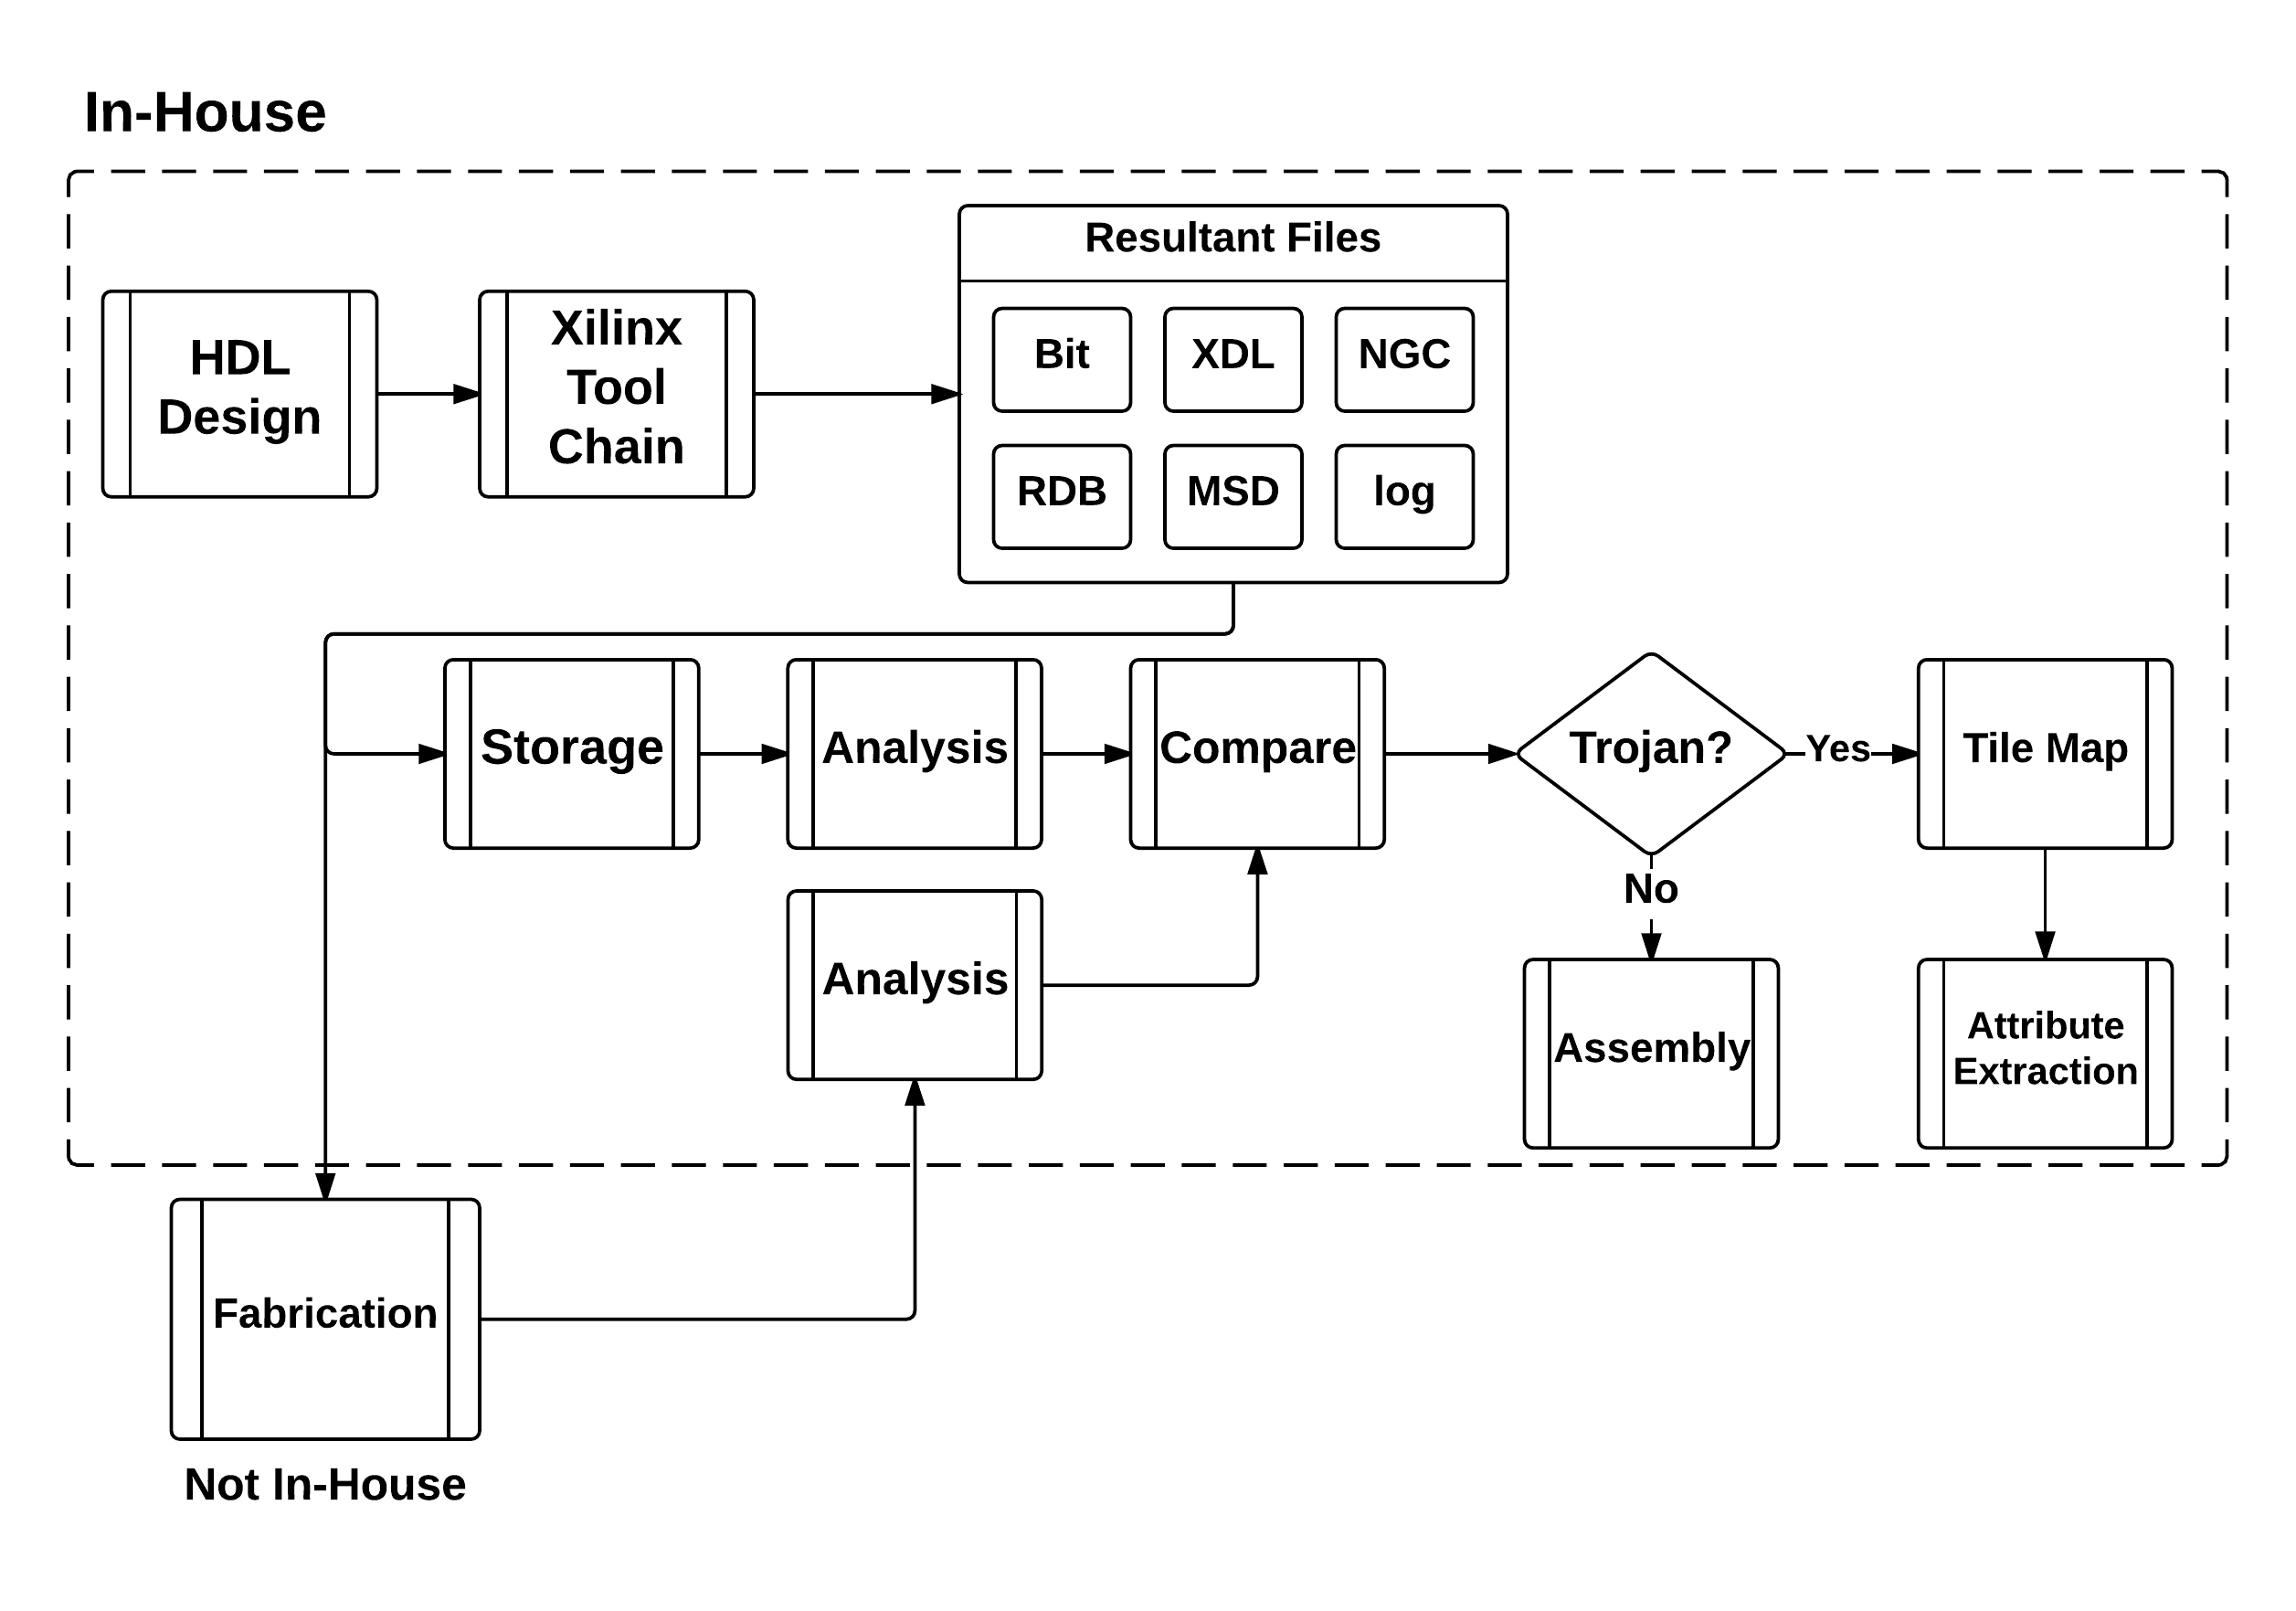
\includegraphics[width=1\linewidth]{Figures/methodologyOverview}
	\caption[Methodology Overview]{Methodology Overview}
	\label{fig:methodologyOverview}
\end{figure}
The resultant files, produced 'in-house' are to be kept in secure storage while a copy is sent to be fabricated; these stored copies are referred to as Golden and assumed to be trojan-free.
Though it is known that the fabrication houses will often attempt to make optimizations on designs, this methodology requires that no such efforts be made.
When the completed batch of fabricated chips are returned the Bitstream is extracted from a sample using the \textit{Xilinx} feature Readback. 
That which is extracted is referred to as the Target Bitstream.
The Golden and Target Bitstreams are analyzed in conjunction to detect differences.
Any discovered differences are then attributed to the corresponding component in the architecture.
Modified components are then related to the user's design using the XDL file.
Finally, the resultant taxonomic description is built and returned to the user.

%%%%%%%%%%%%%%%%%%%%%%%%%%%%%%%
\subsection{Bitstream Analysis} \label{sec:bitstreamComposition}

An FPGA is composed of a matrix of blocks referred to as the gate-array.
Blocks perform functions specified by the configuration they receive from the synthesis process.
The \textit{Xilinx} Bitstream is a binary file composed of a series of 32-bit words organized into 'frames'.
A frame is a string of single bits that span from the top to the bottom of a clock region of a device.
A frame affects every block in a column and multiple horizontally adjacent frames are required to configure an entire column.
Each frame is uniquely identified by a 32-bit address shown in Table~\ref{tbl:frameAddress} and is the smallest addressable element.

%%%%%%%%%%%

\begin{itemize}
	\item BA 0: Logic type.
	\item BA 1: Block Random Access Memory (BRAM).
	\item BA 2: BRAM Interconnect.
	\item BA 3: BRAM non-configuration frame.
\end{itemize}

The Block Address (BA) discerns whether the block type is a logic block, a memory block or memory interconnect.
The Logic block (BA: 0) contains the columns which provide the primary configuration for the device (CLBs, IOBs... etc).
The BRAM columns (BA: 1) initialize the memory for the device while the BRAM Interconnect columns (BA: 2) configure how the logic of the design interacts with the BRAM.

In the case of the Virtex-5 family each clock region is composed of twenty blocks in a column separated by a horizontal clock bus as shown in Fig.~\ref{fig:RowOrder}.
\begin{figure}[h]
	\centering
	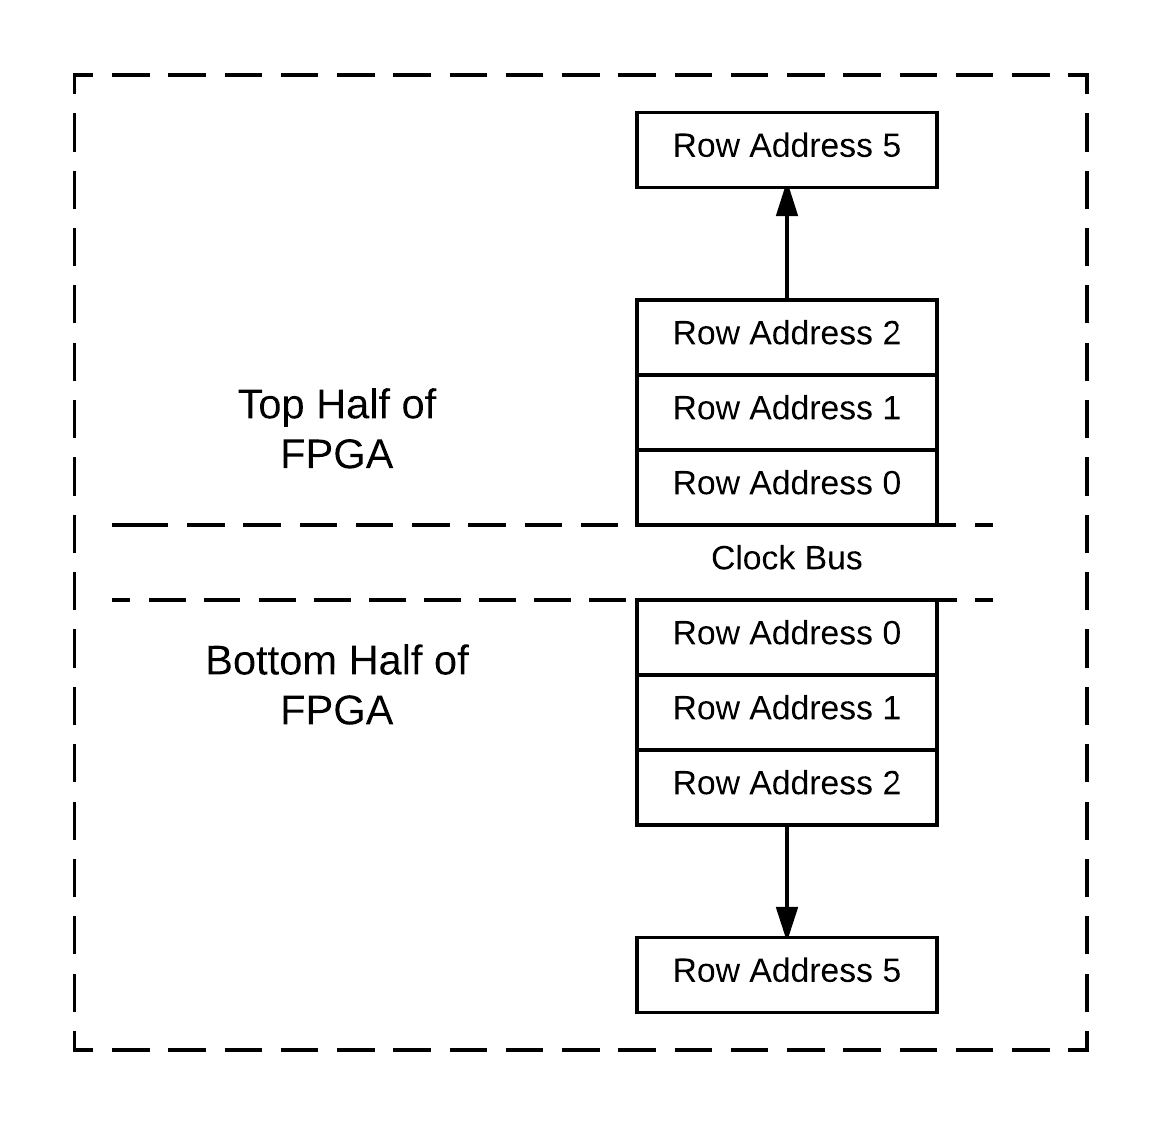
\includegraphics[width=1\linewidth]{Figures/RowOrder}
	\caption[Row Order of Virtex-5 Clock Region]{Row Order of Virtex-5 Clock Region}
	\label{fig:RowOrder}
\end{figure}
Each clock region is given a row value in its address that increments away from the center of the device starting at 0. 
The frame-address includes a Top indicator bit in position 20 that indicates whether the specified row is above or below the center of the device~\cite{virtex5ConfigGuide}.
The major-address specifies the column within the row.
These addresses are numbered from left to right and begin at 0.
The minor-address indicates the frame number within a column. 
Table~\ref{tbl:minorAddressNumbers} provides the number of frames per column type.

In the \textit{Xilinx} jargon, a tile is a conceptual encapsulation of components in the gate-array which perform a specific task.
A block may contain multiple tiles.
A Logic (BA: 0) column of blocks may be one of many types.
As an example, in a Configurable Logic Block (CLB) column, each block consists of an interconnect tile (also known as a Switching Matrix (SM)) on the left, and a CLB tile on the right, as shown in Fig~\ref{fig:column}.
\begin{table}[h]
	\centering
	\caption{Number of Frames (minor-addresses) per Column~\cite{virtex5ConfigGuide}}
	\label{tbl:minorAddressNumbers}
	\begin{tabular}{|c|c|}
		\hline
		Block             & Number Of Frames \\ \hline
		CLB               & 36               \\ \hline
		DSP               & 28               \\ \hline
		BRAM   & 30               \\ \hline
		IOB               & 54               \\ \hline
		Clock             & 4                \\ \hline
	\end{tabular}
\end{table}
\begin{figure}[h]
	\centering
	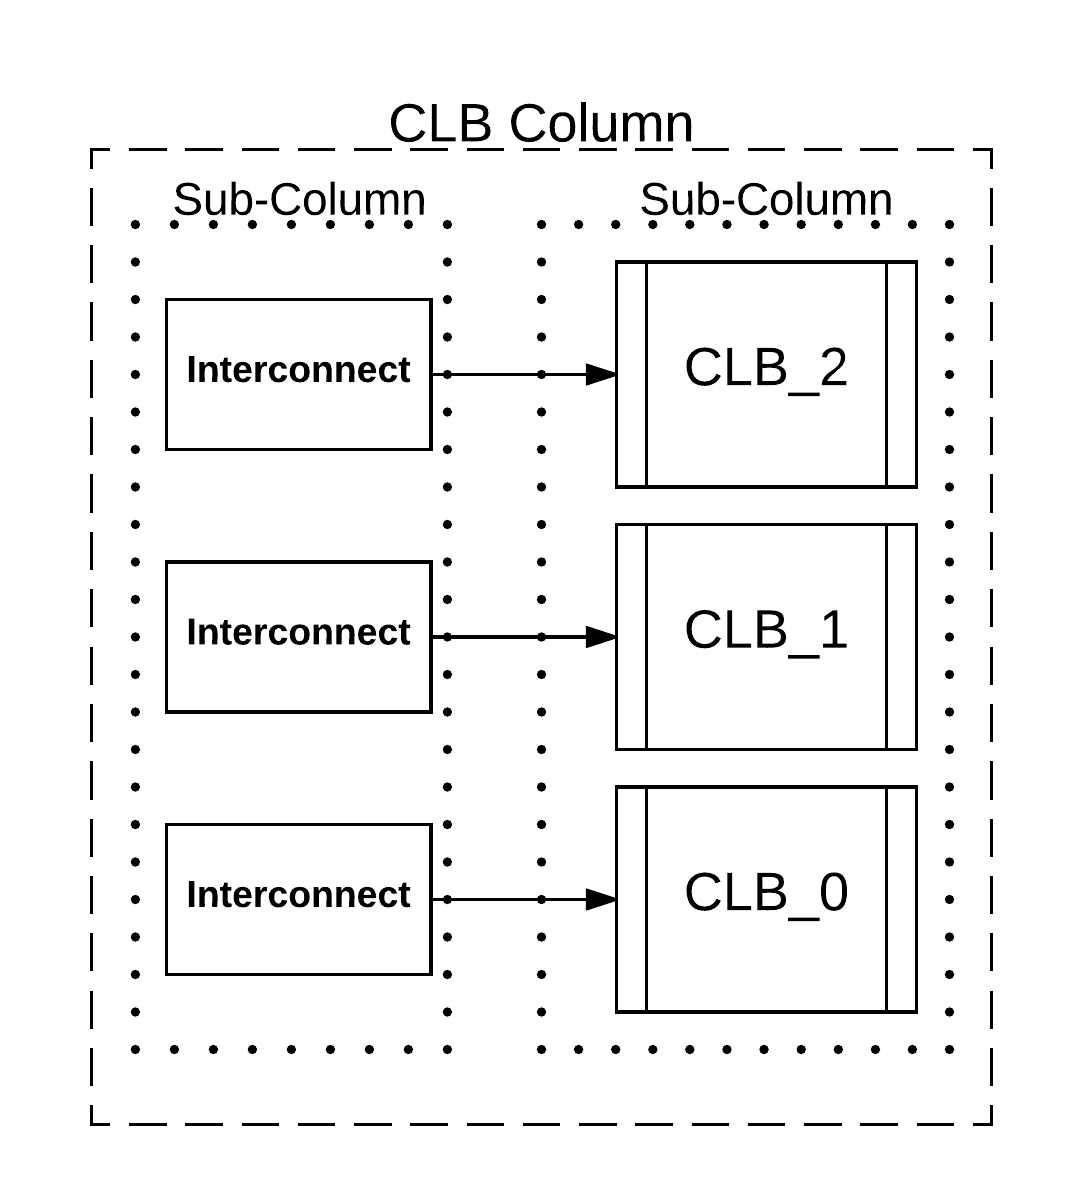
\includegraphics[width=0.8\linewidth]{Figures/column}
	\caption[Column Composition]{Column Composition}
	\label{fig:column}
\end{figure}

The Frames which configure a column are numbered from left to right, starting with 0.  
For the Configurable Logic Block (CLB) column, frames with a minor-address of 0 to 25 configure the interconnect (SM) tile.
Frames numbered 26 and 27 access the Interface for that column. 
The remainder configure the CLB tile~\cite{virtex5ConfigGuide}.
To further understand how frames configure tiles a mapping must be made between each frame and the corresponding tile.
When analyzing the Golden and Target Bitstreams, by understanding how frames configure the blocks of the gate-array, the address of any modified frames can point to exactly which tile has been affected.
A process know as 'Component Mapping' has been developed. 

%%%%%%%%%%%%%%%%%%%%%%%%%%%%%%%
\subsection{Component Mapping} \label{sec:tileMapping}
The format of the configuration Bitstream describes the link between each word in a configuration frame and the component on the device that it configures. 
This format is not publicly released by \textit{Xilinx} as a means of providing security through obscurity.
The FPGA Trojan Detector employs a method referred to as Component Mapping to discern how any discovered modifications affect the device.

When powered-on, the Bitstream is transmitted in frame-address order to populate the dynamic memory in the tiles of the gate-array.
The frame-addressing scheme describes where in the gate-array the frame is destined fairly directly.
As described in section~\ref{sec:bitstreamComposition}, the Block Address (BA) value discerns whether the column type is a logic block column (BA: 0), a Block Random Access Memory (BRAM) column (BA: 1), or a memory interconnect block (BA: 2).
Frames with a BA value of 1 are clearly destined to configure the BRAM and do not need further analysis for the purposes of this method.
Frames with a BA value of 0 or 2 must be mapped more finitely.
The row-address specifies which row of clock-regions the frame is destined, as was seen in Fig.~\ref{fig:RowOrder}.

As an example the Virtex-5 240T has 12 rows~\cite{virtex5ConfigGuide}; its row-address spans from 0-5 and the Top bit in the address indicates whether it is in the top or bottom half of the device in accordance with Fig.~\ref{fig:RowOrder}.
Once the correct clock region is discerned the major-address is used to determine which column the frame configures.
The major-address begins at 0 on the left and counts up towards the number of columns in the row.
Finally, the minor-address is used to determine which sub-column has been modified.
%\subsubsection{Word to Tile Mapping}
In the \textit{Xilinx} jargon, a tile is a conceptual encapsulation of components in the gate-array which perform a specific task.
A block may contain multiple tiles.

As an example, in a Configurable Logic Block (CLB) column, each block consists of an interconnect tile (also known as a Switching Matrix (SM)), an interface tile, and a CLB tile.
The Frames which configure a column have a minor-address numbered from left to right, starting with 0.
Frames with a minor-address from 0 to 25 configure the interconnect (SM).
Frames numbered 26 and 27 access the interface tile and the remainder configure the CLB tile~\cite{virtex5ConfigGuide}.
\begin{figure}[h]
	\centering
	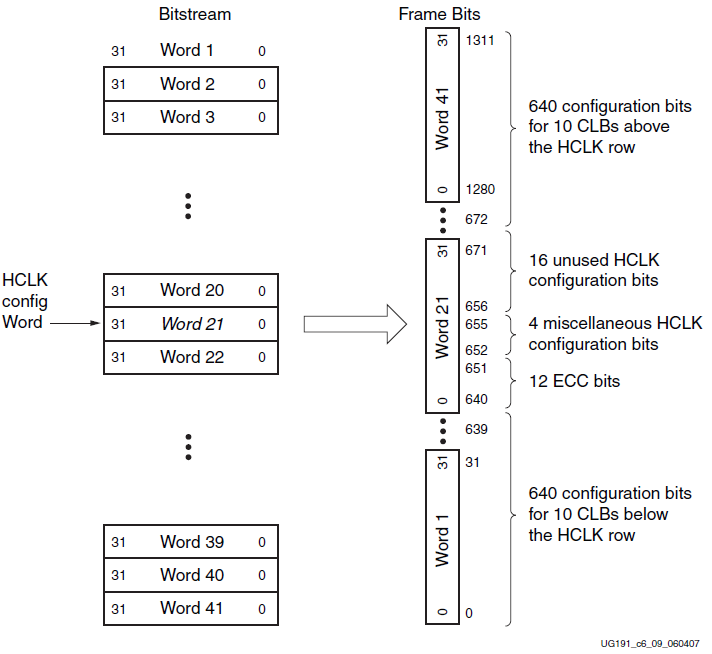
\includegraphics[width=0.96\linewidth]{Figures/frameTileMap}
	\caption[Configuration Words in the Bitstream~\cite{virtex5ConfigGuide}]{Configuration Words in the Bitstream~\cite{virtex5ConfigGuide}}
	\label{fig:frameTileMap}
\end{figure}

Figure~\ref{fig:frameTileMap} shows how a frame is composed of 41 words which can be thought of as a vertical stack that aligns within a column.
Similarly, a component column consists of a stack of blocks; there are 20 blocks per CLB column, 40 per IOB column, 4 per BRAM and so on.
The configuration words within a frame align with the physical blocks of the column.
To compute which word corresponds to which component a series of equations has been developed.
First, Equation~\ref{eqn:numWordsPerBlock} is used to compute the number of 32-bit words that span each block.
\begin{equation} \label{eqn:numWordsPerBlock}
n = (W - C) + B
\end{equation}

where:
\begin{conditions}
	n     &  Number of Words per Block \\
	W     &  Number of 32-bit words per frame \\   
	C     &  Number of clock words per frame \\
	B     &  Number of blocks per column
\end{conditions}
%\normalsize
Referring to Fig~\ref{fig:column}, physical components are numbered from the bottom up while, as seen in Fig~\ref{fig:frameTileMap}, configuration words are numbered from the top of the column down.
This ordering pattern results in Equation~\ref{eqn:getTileNumber}.
The result of Equation~\ref{eqn:numWordsPerBlock} and the modified word's position in the frame are used to determine which block the modification affected.
\begin{equation} \label{eqn:getTileNumber}
i = B - \floor*{\frac{w}{n}}
\end{equation}
%\ConditionSize
where:
\begin{conditions}
	i     &  Block number in column\\
	B     &  Number of blocks per column \\
	w     &  Modified Word's number in the frame\\
	n     &  Number of Words per Block 
\end{conditions}
%\normalsize
By using equations~\ref{eqn:numWordsPerBlock} and~\ref{eqn:getTileNumber} and knowing how the minor-address relates to the column it is possible to link any modifications in the Bitstream to its corresponding tile in the device.

%%%%%%%%%%%%%%%%%%%%%%%
%\subsection{Design Analysis}

\section{Determining Trojan Attributes} \label{sec:trojanAttributes}
The taxonomy in~\cite{samerAttribute} provides a series of thirty-three attributes which a trojan may or may not posses.
Though it is desirable to be able to observe and directly extract the attributes a trojan possesses it is not always possible. 
In~\cite{samerAttribute} a matrix, $\mathbf{R}$, is provided which describes the relationships between each of the thirty-three attributes in the taxonomy.
When it is not possible to directly determine the presence of certain attributes, this relation matrix is used to infer their existence.
The analysis stage of the automated trojan detection technique provided by this work begins by extracting those attributes that are directly observable then using matrix $\mathbf{R}$ to infer the existence of the remainder. 

%%%%%%%%%%%%%%%%%%%%%%%
\subsection{Observed Location Attributes}
The presence of attributes in the \textit{Location} category are directly observable from the results of the component mapping method described in section~\ref{sec:tileMapping}.
\textit{Xilinx} tiles conform to purpose-specific groups or block types.
These block-types perform actions which pertain directly to \textit{Location} category attributes
Attributes can be awarded for the following traits: 
\begin{enumerate}
	\item The \textbf{Processor} attribute pertains to the core functionality of the design logic. It can be awarded for the presence of a modified CLB tile or Interconnect tile in a trojan.
	\item The \textbf{Memory} attribute can be awarded for the presence of modified BRAM components.
	\item The \textbf{Input-Output} attribute can be awarded for presence of modified IOB tiles.
	\item The \textbf{Power Supply} attribute can be awarded for the presence of modified interface or configuration tiles.
	\item The \textbf{Clock Grid} attribute can be awarded for modified clock tiles.
\end{enumerate}

%%%%%%%%%%%%%%%%%%%%%%%
\subsection{Scatter Score Method} \label{sec:scatterScore}
The gate-array configuration of components in \textit{Xilinx} FPGAs allows for an analytical method of determining attributes in the \textit{Physical Layout} category.
The "Scatter Score" method uses the grid coordinates of components to derive a numerical score rating for the size, position, and augmentation of configured tiles.
Tiles are assigned global coordinates that represent their horizontal and vertical positions within the gate array denoted $x$ and $y$ respectively. 
These values can then be used to strongly infer the presence of \textit{Physical Location} attributes.
The following series of steps are first performed on the Golden design, followed by the Target; a comparison is then performed and a score is determined.

The Scatter Score method begins by determining the total number of configured tiles in the design.
Equation~\ref{eqn:numConfiguredTiles} is used and the total is stored for subsequent use.
\begin{equation} \label{eqn:numConfiguredTiles}
n = \sum_{x = 0}^{X}\sum_{y = 0}^{Y}T_{xy}
\end{equation}
where:
\begin{conditions}
	n     &  Number of all configured tiles \\
	X     &  The column width of the gate-array \\   
	Y     &  The number of rows of the gate-array \\
	T     &  A configured tile
\end{conditions}

Then, the average horizontal and vertical positions are computed using Equations~\ref{eqn:xAverage} and~\ref{eqn:yAverage}.
Combined, these averages are used in conjunction to form the Position Median as seen in Equation~\ref{eqn:positionMedian}.
The Position Median provides an easy to interpret centralization of the design. 
Activation or deactivation of tiles by a trojan will shift the position median; this provides valuable insight into which \textit{Physical Layout} category attributes the trojan possesses.
\begin{equation} \label{eqn:xAverage}
a_x = \frac{1}{n}\sum_{x=0}^{n}T_x
\end{equation}
\begin{equation} \label{eqn:yAverage}
a_y = \frac{1}{n}\sum_{y=0}^{n}T_y
\end{equation}
\begin{equation} \label{eqn:positionMedian}
M_{xy} = (a_x,~a_y)
\end{equation}
where:
\begin{conditions}
	$$a_x$$     &  The average x coordinate of configured tiles \\   
	$$a_y$$     &  The average y coordinate of configured tiles \\
	$$T_x$$     &  The x coordinate of a configured tile \\
	$$T_y$$	    &  The y coordinate of a configured tile \\
	$$M_{xy}$$     &  The Position Median
\end{conditions}
%\noindent\begin{minipage}{.5\linewidth}
%	\begin{equation} \label{eqn:xAverage}
%	a_x = \frac{1}{n}\sum_{x=0}^{n}T_x
%	\end{equation}
%\end{minipage}%
%\begin{minipage}{.5\linewidth}
%	\begin{equation} \label{eqn:yAverage}
%	a_y = \frac{1}{n}\sum_{y=0}^{n}T_y
%	\end{equation}
%\end{minipage}
%\\
%\noindent\begin{minipage}{.5\linewidth}
%	\begin{equation} \label{eqn:stdDevX}
%	\sigma_x = \sqrt{\frac{1}{n}\sum_{x = 0}^{X}(x_i - a_x)^2)}
%	\end{equation}
%\end{minipage}%
%\begin{minipage}{.5\linewidth}
%	\begin{equation} \label{eqn:stdDevY}
%	\sigma_y = \sqrt{\frac{1}{n}\sum_{y = 0}^{Y}(y_i - a_y)^2)}
%	\end{equation}
%\end{minipage}
Once the Position Median has been computed the average values $a_x$ and $a_y$ can be used to determine the standard deviation of the position of tiles via Equations~\ref{eqn:stdDevX} and~\ref{eqn:stdDevY}.
These values are then combined to create the Scatter Score for the design, shown in Equation~\ref{eqn:scatterScore}.
Again, the activation or deactivation of tiles will alter the value of the Scatter Score providing valuable insight into the clustering of a trojan.
\begin{equation} \label{eqn:stdDevX}
\sigma_x = \sqrt{\frac{1}{n}\sum_{x = 0}^{X}(x_i - a_x)^2)}
\end{equation}
\begin{equation} \label{eqn:stdDevY}
\sigma_y = \sqrt{\frac{1}{n}\sum_{y = 0}^{Y}(y_i - a_y)^2)}
\end{equation}
\begin{equation} \label{eqn:scatterScore}
S_{xy} = (\sigma_x,~\sigma_y)
\end{equation}
where:
\begin{conditions}
	$$\sigma_x$$ & Standard deviation of the x coord. of configured tiles \\
	$$\sigma_y$$ & Standard deviation of the y coord. of configured tiles \\
	$$T_x$$     &  The x coordinate of a configured tile \\
	$$T_y$$	    &  The y coordinate of a configured tile \\
	$$S_{xy}$$     &  The Scatter Score
\end{conditions}
The \textit{Physical Location} category contains six attributes.
These six can be considered three pairs; a trojan exhibits one attribute from each pair. 
\begin{enumerate}
	\item \textbf{Large or Small} (attributes 23 or 24): According to~\cite{samerAttribute}, small trojans are defined as those that are nearly impossible to detect via power consumption. From this it can be said that 'small' trojans occupy minimal resources. It was found that trojans where the number of reconfigured tiles is less than 5\% of the number of tiles in the golden design should be considered small. Other wise they are attributed as large.
	\item \textbf{Changed Layout or Augmented} (attributes 25 or 26): A 'changed layout' trojan is such that only tiles that are configured by the golden design are reconfigured. An augmented trojan is where additional layout is added. The presence of 'activated' or 'deactivated' tiles indicates an augmented trojan. 
	\item \textbf{Clustered or Distributed} (attributes 27 or 28): It was found that a trojan should be considered clustered when the standard deviation of the reconfigured tile positions is less than 15\%; distributed otherwise.
\end{enumerate}
\subsection{Insertion and Abstraction Attributes}
The linear nature of the manufacturing life-cycle implies a propagation of effects.
For the purposes of this method it is assumed that the only non-trustworthy stage in the life-cycle is fabrication.
In other words, the trojan was inserted in the third-party fabrication stage.
Due to the propagating nature of the life-cycle the effects of the modifications made in the fabrication stage (attribute 3) are felt in the testing (attribute 4) and assembly (attribute 5) stages.
Hence, it can be said that this trojan possesses insertion category attributes 3, 4 and 5.

FPGA designs are made with a HDL.
These languages dictate component arrangement in the Registry Transfer Level (RTL) abstraction level.
Hence it can be said that trojans occurring in FPGAs take place in the System (attribute 6) and RTL (attribute 7) abstraction levels.

\subsection{Relation Matrix Use} \label{sec:matrixUse}
Attributes which are not directly observable can be inferred using a systematic method of analyzing the rows and columns of the relation matrix presented in~\cite{samerAttribute}.
The FPGA Trojan Detector takes the attributes it is able to directly observe and uses them as input to this process.
A thorough description of this method is given in~\cite{samerDissertation} and~\cite{meCategorization}.

%%%%%%%%%%%%%%%%%%%%%%%%%%%%%%%%%
\section{FPGA Trojan Detector} \label{sec:implementation}
The FPGA Trojan Detector can provide manufacturers additional security that takes only minutes to complete; the analysis requires only a few button clicks.
It was built to be a stand-alone application; it is light-weight, cross platform and does not require a complex installation.
\subsection{Technologies Used}
\subsubsection{\textit{Xilinx}}
\textit{Xilinx} is one of the two largest manufacturers of FPGAs; their devices are considerably more popular than their competitors.

\subsubsection{Java} \label{sec:java}
FPGA Trojan Detector was written in Java~\cite{java} primarily in order to interface with the Application Programming Interface (API) known as RapidSmith which is described in section~\ref{sec:rapidSmith}.
However, Java additionally allows the FPGA Trojan Detector to be a compact, cross-platform application.
The custodians of the Java language, Sun Microsystems, promote the slogan 'write-once, run anywhere'. 
The Java language provides a native Graphical User-Interface (GUI) toolkit known as \textit{Swing}~\cite{swing}.
\textit{Swing} is an API that is part of Oracle's Java Foundation Classes; in other words it is readily available to all users of Java.

\subsubsection{\textit{RapidSmith}} \label{sec:rapidSmith}
RapidSmith is an API written in Java that enables Computer Aided Design (CAD) tool creation for \textit{Xilinx} FPGAs~\cite{rapidSmith}.
Its purpose is to be used as a rapid prototyping platform for experimentation and research.
It was chosen as a supporting library for the FPGA Trojan Detector for several reasons.
First, the code base provides a series of class structures that astutely mirror the architecture of \textit{Xilinx} devices.
Secondly, it provides ready-made tools for extracting the configuration frames from Bitstream files. 
Bitstream files are long binary sequences, without the tools provided by RapidSmith the analysis of these files becomes an arduous task.

\textit{Xilinx} provides a tool capable of generating large text files which fully describe every facet of a chosen device.
Known as XDLRC files, the FPGA Trojan Detector requires these descriptions to perform the Component Mapping described in section~\ref{sec:tileMapping}
These description files can reach 20GB or more in size making them incredibly inefficient to analyze.
The most important and beneficial feature of RapidSmith is that the creators have developed a means of condensing XDLRC files into a greatly compressed format referred to as a 'database' file.
This compression reduces a 20GB XDLRC to a 7MB database file which allows for efficient analysis.

%%%%%%%%%%%%%%%%%%%%%%%%%%%%%%%%%

\begin{table*}[t!]
	\setlength{\tabcolsep}{3pt}
	\centering
	\caption{Outputs of the Circuits in Figs.~\ref{fig:userAuthenticationCircuit} and \ref{fig:userAuthenticationCircuitTrojan}~\cite{samerAttribute}}
	\label{tbl:trojanOutputs}
	\begin{tabular}{CC|C|C|C|C|C||C|C|C|C|C|C|C|C||C|C|C|C|C|C|C|C|}
		\cline{3-23}
		&  & \multicolumn{5}{c||}{Inputs} & \multicolumn{8}{c||}{Circuit A} & \multicolumn{8}{c|}{Circuit B} \\ \cline{3-23}
		&  & X_1 & X_2 & X_3 & X_4 & X & Z_1 & Z_2 & Z_3 & Z_4 & Z_5 & Z_6 & Z_7 & F(x) & Z_1 & Z_2 & Z_3 & Z_4 & Z_5 & Z_6 & Z_7 & F(x) \\ \hline
		\multicolumn{1}{|c|}{\multirow{10}{*}{\rotatebox[origin=c]{90}{Inputs}}} & I_0 & 0 & 0 & 0 & 0 & 0 & 0 & 0 & 0 & 0 & 0 & 0 & 0 & 0 & 0 & 0 & 0 & 0 & 0 & 0 & 0 & 0 \\ \cline{2-23}
		\multicolumn{1}{|c|}{} & I_1 & 0 & 0 & 0 & 1 & 1 & 0 & 0 & 0 & 0 & 0 & 0 & 1 & 1 & 0 & 0 & 0 & 0 & 0 & 0 & 1 & 1 \\ \cline{2-23}
		\multicolumn{1}{|c|}{} & I_2 & 0 & 0 & 1 & 0 & 2 & 0 & 0 & 0 & 0 & 1 & 0 & 0 & 4 & 0 & 0 & 0 & 0 & 1 & 0 & 0 & 4 \\ \cline{2-23}
		\multicolumn{1}{|c|}{} & I_3 & 0 & 0 & 1 & 1 & 3 & 0 & 0 & 0 & 1 & 0 & 0 & 1 & 9 & 0 & 0 & 0 & 1 & 0 & 0 & 1 & 9 \\ \cline{2-23}
		\multicolumn{1}{|c|}{} & I_4 & 0 & 1 & 0 & 0 & 4 & 0 & 0 & 1 & 0 & 0 & 0 & 0 & 16 & 0 & 0 & 1 & 0 & 0 & 0 & 0 & 16 \\ \cline{2-23}
		\multicolumn{1}{|c|}{} & I_5 & 0 & 1 & 0 & 1 & 5 & 0 & 0 & 1 & 1 & 0 & 0 & 1 & 25 & 0 & 0 & 1 & 1 & 0 & 0 & 1 & 25 \\ \cline{2-23}
		\multicolumn{1}{|c|}{} & I_6 & 0 & 1 & 1 & 0 & 6 & 0 & 1 & 0 & 0 & 1 & 0 & 0 & 36 & 0 & 1 & 0 & 0 & 1 & 0 & 0 & 36 \\ \cline{2-23}
		\multicolumn{1}{|c|}{} & I_7 & 0 & 1 & 1 & 1 & 7 & 0 & 1 & 1 & 0 & 0 & 0 & 1 & 49 & 0 & 1 & 1 & 0 & 0 & 0 & 1 & 49 \\ \cline{2-23}
		\multicolumn{1}{|c|}{} & I_8 & 1 & 0 & 0 & 0 & 8 & 1 & 0 & 0 & 0 & 0 & 0 & 0 & 64 & 1 & 0 & 0 & 0 & 0 & 0 & 0 & 64 \\ \cline{2-23}
		\multicolumn{1}{|c|}{} & I_9 & 1 & 0 & 0 & 1 & 9 & 1 & 0 & 1 & 0 & 0 & 0 & 1 & 81 & 1 & 0 & 1 & 0 & 0 & 0 & 1 & 81 \\ \hline
		\multicolumn{1}{|c|}{\multirow{6}{*}{\rotatebox[origin=c]{90}{Undefined}}} & I_{10} & 1 & 0 & 1 & 0 & 10 & 1 & 0 & 0 & 0 & 1 & 0 & 0 & 68 & 1 & 1 & 0 & 0 & 1 & 0 & 0 & 100 \\ \cline{2-23}
		\multicolumn{1}{|c|}{} & I_{11} & 1 & 0 & 1 & 1 & 11 & 1 & 0 & 1 & 1 & 0 & 0 & 1 & 89 & 1 & 1 & 1 & 1 & 0 & 0 & 1 & 121 \\ \cline{2-23}
		\multicolumn{1}{|c|}{} & I_{12} & 1 & 1 & 0 & 0 & 12 & 1 & 1 & 1 & 0 & 0 & 0 & 0 & 112 & 1 & 0 & 1 & 0 & 0 & 0 & 0 & 80 \\ \cline{2-23}
		\multicolumn{1}{|c|}{} & I_{13} & 1 & 1 & 0 & 1 & 13 & 1 & 1 & 1 & 1 & 0 & 0 & 1 & 121 & 1 & 0 & 1 & 1 & 0 & 0 & 1 & 89 \\ \cline{2-23}
		\multicolumn{1}{|c|}{} & I_{14} & 1 & 1 & 1 & 0 & 14 & 1 & 1 & 0 & 0 & 1 & 0 & 0 & 100 & 1 & 1 & 0 & 0 & 1 & 0 & 0 & 100 \\ \cline{2-23}
		\multicolumn{1}{|c|}{} & I_{15} & 1 & 1 & 1 & 1 & 15 & 1 & 1 & 1 & 0 & 0 & 0 & 1 & 113 & 1 & 1 & 1 & 0 & 0 & 0 & 1 & 113 \\ \hline
	\end{tabular}
\end{table*}
\section{Results} \label{sec:results}
To demonstrate its potential, FPGA Trojan Detector has been tested using a series of benchmarks.
In addition, a website known as the Hardware Trojan System~\cite{meCategorization} (HTS) was used to further visualize the results of the benchmark analysis.
The HTS provides a unique tool know as the Classification web tool which accepts a list of taxonomic attributes as input and generates a directed graph.
This graph allows for easy observation of how each attribute inter-relates and affects one another.

%%%%%%%%%%%%%%%%%%%
\subsection{Priority Decoder} \label{sec:priorityDecoder}
The FPGA Trojan Detector was first tested using a small 'Priority Decoder' circuit presented by F. Brglez and H. Fujiwara
in~~\cite{iscas85}.
The provided verilog code for the decoder benchmark was synthesized on a Virtex-5 XC5VLX155 and the generated Bitstream and XDL files were acquired.
The priority decoder Bitstream file was fed to both the Golden and Target inputs to the FPGA Trojan Detector.
Feeding the same Bitstream file to both inputs replicates the occurrence where the third-party fabrication house made no modifications; the Bitstream extracted from the Target device is exactly the same as the Golden.
It is expected that the FPGA Trojan Detector returns a result indicating that there is no trojan present.
The FPGA Trojan Detector successfully analyzed the Bitstreams and determined that there was no trojan present, as expected.

\subsection{User Authentication Circuit} \label{sec:userAuthentication}
Consider a circuit designed to compute a function $F(x)$ for a system to authenticate user-password pairs $x$ and $F(x)$.
The system performs the arithmetic operation $F(x) = x^2$ to validate users; the customer wishes to provide access to ten clients labeled $I_0$ to $I_9$.
To identify all ten clients, four input bits are required, $x_1$ to $x_4$.
In consequence, the largest valid output of $F(x) = x^2$ is $81$ meaning that seven bits are required for output. 
These outputs are labeled $Z_1$ to $Z_7$ and are illustrated in Fig.~\ref{fig:userAuthenticationCircuit}.
A trojan can be inserted into this circuit as shown in Fig.~\ref{fig:userAuthenticationCircuitTrojan} (referred to as a backdoor trojan).
\begin{figure}[h]
	\centering
	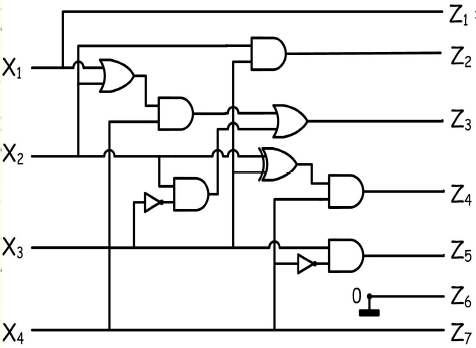
\includegraphics[width=0.7\linewidth]{Figures/circuit1}
	\caption{A Simple User Authentication Circuit}
	\label{fig:userAuthenticationCircuit}
\end{figure}
\begin{figure}[h]
	\centering
	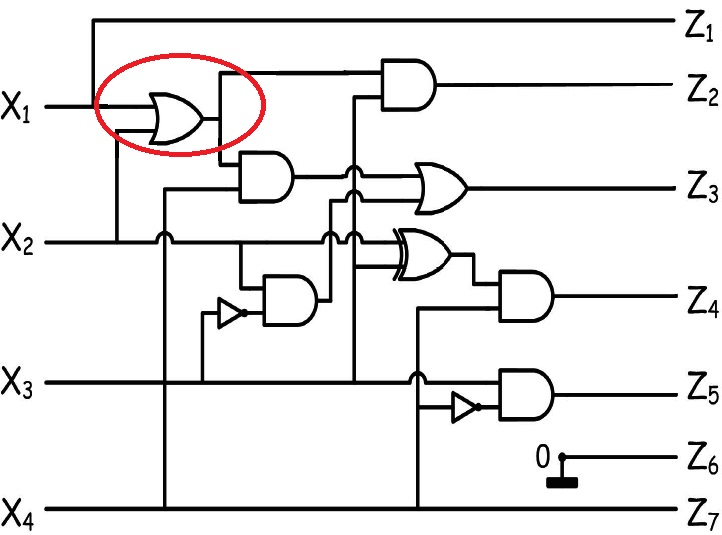
\includegraphics[width=0.7\linewidth]{Figures/circuit2}
	\caption{The Back-door Trojan}
	\label{fig:userAuthenticationCircuitTrojan}
\end{figure}

The outputs of the original and infected circuits are compared in Table~\ref{tbl:trojanOutputs}.
A simple test will show that the circuit outputs the desired $F(x) = x^2$ for each of the users.
However, upon closer inspection it is noted that the inputs corresponding to $x = 10$ to $x = 15$ are not used; there are no clients occupying those identifications.
These unused inputs are referred to as 'dont-cares' (DC), meaning that it is not important to the function of the circuit what their corresponding output is.
Don't-care cases are a typical vulnerability which can be exploited by an attacker.
Under the 'Circuit A' column of Table~\ref{tbl:trojanOutputs} it can be seen that $I_{10}$ and $I_{11}$ produce results 68 and 89 respectively.
These results are not correct according to $F(x) = x^2$.
This is an intended result by the circuit designer to add security for these don't care conditions.
If an attacker is able to make the modification in Fig.~\ref{fig:userAuthenticationCircuitTrojan}, inputs $10$ and $11$ will now produce results 100 and 121 which are correct according to $F(x) = x^2$.
This can be seen under the 'Circuit B' column of Table~\ref{tbl:trojanOutputs}.
The attacker has now built a 'back-door' into the circuit.
The original 10 users' authentication is not altered but inputs 10 and 11 provide unauthorized access.
\begin{figure*}[b]
	\centering
	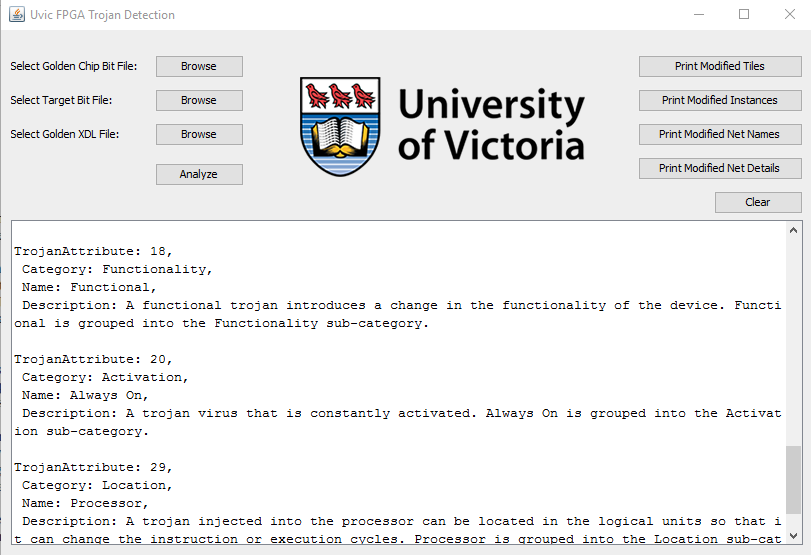
\includegraphics[width=0.7\linewidth]{Figures/backDoorResult}
	\caption[Results of The Authentication Circuit Trojan Detection]{Results of The Authentication Circuit Trojan Detection}
	\label{fig:backDoorResult}
\end{figure*}

The circuits shown in Figures~\ref{fig:userAuthenticationCircuit} and~\ref{fig:userAuthenticationCircuitTrojan} were implemented and synthesized on a Virtex-5 240T  (XC5VSX240T).
The resultant Bitstreams were input to the FPGA Trojan Detector and the analysis detected a trojan.
It output the following list of attributes as can be partially seen in Figure~\ref{fig:backDoorResult}.

\begin{itemize}
	\item Attribute 3: Fabrication
	\item Attribute 4: Testing
	\item Attribute 5: Assembly
	\item Attribute 6: System
	\item Attribute 7: RTL
	\item Attribute 12: Change in Functionality
	\item Attribute 17: Combinational
	\item Attribute 18: Functional
	\item Attribute 20: Always On
	\item Attribute 24: Small
	\item Attribute 26: Augmented
	\item Attribute 27: Clustered
	\item Attribute 29: Processor
\end{itemize}

As expected the results state that the trojan was inserted in the Fabrication phase (3); it is the earliest stage in the 'insertion' phase produced indicating it as the source.
The effects of this modification propagate to the Testing (4) and Assembly (5) phases as expected.
The modifications reach both the System (6) and Registry Transfer Level (RTL) (7) abstraction levels.
Since the modifications were made using the schematic designer provided by \textit{Xilinx} which works in the RTL level, these results are as expected.
The results indicate that the trojan Changes Functionality (12). 
This agrees with the modification to the values listed in Table~\ref{tbl:trojanOutputs}.
The trojan does not take affect over multiple clock cycles; this indicates it is composed of only Combinational (17) circuitry which is reflected in the results.
The trojan did not modify power levels or operation configurations, only design configurations.
This indicates that the trojan can be described as Functional (18), not Parametric (19); this agrees with the results.
Since the modification made a permanent alteration to the internal wiring of the circuit it can be said to be Always On (20).

The modified values for input $x=10$ or $x=11$ are always available and not activated.
This is consistent with the returned results.
The trojan changed only minor routing configurations in the circuit designs, this required the alteration of only a few tiles.
The new route required the activation of tiles which were not active in the Golden design; further, all of the modified tiles are nearby those in the Golden design. 
With these observations it can be said that this trojan exhibits Physical Layout attributes Small (24), Augmented (26) and Clustered (28). 
All of the expected Physical Layout attributes were correctly determined by the Scatter Score method of section~\ref{sec:scatterScore}.
Finally, all of the tiles modified by the trojan belong to major block type 0: Logic Type.
These tiles only affect the internal processing of the circuit.
No IOB, Clock or BRAM tiles were modified.
This is reflected by the fact that only Location attribute, Processor (29), was returned by the analysis.
The results observed by the experiment conformed with the experiments expectations demonstrating the accuracy of the method.
The entire analysis takes less than a minute to perform.
\begin{figure}[h]
	\centering
	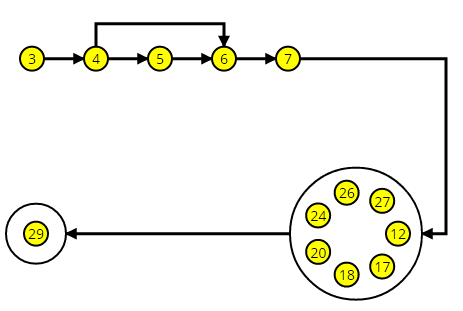
\includegraphics[width=0.91\linewidth]{Figures/backDoorVisual}
	\caption[Directed Graph of Back-Door Trojan generated by the Hardware Trojan System]{Directed Graph of Back-Door Trojan generated by the Hardware Trojan System}
	\label{fig:backDoorVisual}
\end{figure}
The attributes found to describe the back-door trojan in the User Authentication Circuit are entered into the Hardware Trojan System in the Classification tool.
The matrix $\mathbf{R}$ is automatically analyzed and the visualization shown in Figure~\ref{fig:backDoorVisual} is presented.

\subsection{AES-T100} \label{sec:aesT100}
In 2013 H.~Salmani, M.~Tehranipoor and R.~Karri published a discussion on the design and development of FPGA trojan benchmarks.
They collaboratively developed a series of verilog, VHDL and virtual machines that demonstrated effective creation of testable benchmarks.
They took the benchmarks they created and published them on a website they created called \textit{Trust-Hub}.
The benchmarks provided are organized by a taxonomy they proposed in~\cite{trustHubPaper}.
Their taxonomy is slightly different than the one used by the FPGA Trojan Detector which was proposed in~\cite{samerAttribute}, however the two are conceptually similar.
To demonstrate the efficacy of the FPGA Trojan Detector a benchmark named 'AES-T100' was chosen. 
The supporting documents describe this trojan as follows:
\begin{displaycquote}{trusthubWebsite}
	The Trojan leaks the secret key from a cryptographic chip running the AES algorithm through a covert channel. The channel adapts the concepts from spread spectrum communications (also known as Code-Division Multiple Access (CDMA)) to distribute the leakage of single bits over many clock cycles. The Trojan employs this method by using a pseudo-random number generator (PRNG) to create a CDMA code sequence, the PRNG initialized to a predefined value. The code sequence is then used to XOR modulate the secret information bits. The modulated sequence is forwarded to a leakage circuit (LC) to set up a covert CDMA channel in the power side-channel. The LC is realized by connecting eight identical flip-flop elements to the single output of the XOR gate to mimic a large capacitance.
\end{displaycquote}
\begin{figure*}[t]
	\centering
	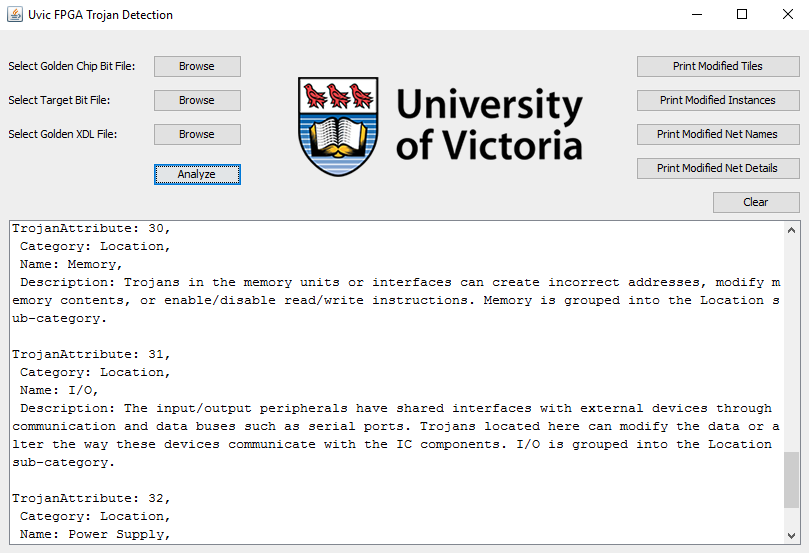
\includegraphics[width=0.7\linewidth]{Figures/aesResult}
	\caption[Results of Analysis on the AES-T100 Benchmark]{Results of Analysis on the AES-T100 Benchmark}
	\label{fig:aesResult}
\end{figure*}
From the description it is reasonable to expect certain results from the FPGA Trojan Detector.
The description states that the trojan 'leaks the secret key'.
From this we should expect our results to contain Effect attribute Information Leakage (13).
Information being leaked from a device will need a means to be transmitted to the attacker.
Location attribute IO (31) may be observed.
It then states that it leaks 'single bits over many clock cycles'. 
This suggests that the trojan exhibits some form of Sequential Logic (16).
This may or may not require modification to clock tiles; Location attribute Clock Grid (33) may be observed. 
It then states that the PRNG is initialized to a predefined value; initialization requires the value be stored in memory. 
Location attribute Memory (30) should be expected.
The trojan then uses a 'power side-channel' as a communication channel.
This will require modification to power tiles; Location attribute Power Supply (32) should be expected.

The source code for the Golden and Target designs were downloaded from \textit{trust-hub.org} and synthesized on a Virtex-5 240T  (XC5VSX240T).
The analysis results were successfully found by the system as seen in Figure~\ref{fig:aesResult}.


The FPGA Trojan Detector output the following attributes:
\begin{itemize}
	\item Attribute 3: Fabrication
	\item Attribute 4: Testing
	\item Attribute 5: Assembly
	\item Attribute 6: System
	\item Attribute 7: RTL
	\item Attribute 13: Information Leakage
	\item Attribute 16: Sequential
	\item Attribute 18: Functional
	\item Attribute 20: Always On
	\item Attribute 24: Large
	\item Attribute 26: Augmented
	\item Attribute 27: Distributed
	\item Attribute 29: Processor
	\item Attribute 30: Memory
	\item Attribute 31: IO
	\item Attribute 32: Power Supply
	\item Attribute 33: Clock Grid
\end{itemize}

Again, it is assumed that this trojan was inserted during the fabrication phase; due to this the effects propagate to the Testing (4) and Assembly (5) phases.
Again, the trojan resides in the System (6) and RTL (7) abstraction levels as was expected.
Attributes 13, 16, 30, 31, 32 and 33 appear in the analysis results as expected.
The Scatter Score method describes this trojan as Large, Augmented and Distributed. 
These results seem to correspond well with the description. 
The addition of the leakage circuit and the PRNG would be non-trivial addenda likely requiring the activation of considerable resources resulting in attribute Augmented (26).
Due to their complexity these added circuits will most likely need to be placed away from the Golden resources causing attribute Distributed (27).

The resultant attributes are input to the Hardware Trojan System.
Again, the matrix $\mathbf{R}$ is automatically analyzed and the visualization shown in Figure~\ref{fig:aesVisual} is presented.
\begin{figure}[h]
	\centering
	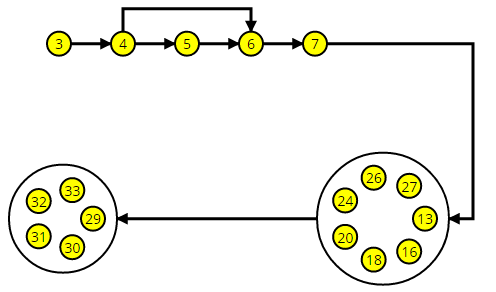
\includegraphics[width=0.91\linewidth]{Figures/aesVisual}
	\caption{Directed Graph of AES Circuit Trojan generated by the Hardware Trojan System}
	\label{fig:aesVisual}
\end{figure}

%%%%%%%%%%%%%%%%%%%%%%%%%%%%%%%%%%%%%%%%%%%%%%%%%%%%%%%%
\section{Conclusion} \label{sec:conclusion}
Configuration Bitstreams are enormous strings of binary data.
To the human reader this information means nothing.
To an FPGA, however, this data is everything.
Every conceivable design, and every possible trojan is contained within the Bitstream.
Yet, due to the shear volume of information within it, it has not previously been a common subject of study.
With the new methodology presented in this work, integrated-circuit manufacturers that use FPGAs will have an additional tool to ensure that their products operate as expected.
Trojans inserted into FPGA designs can now be easily detected and described.
Using the FPGA Trojan Detector takes only a few button clicks on the user-interface.
Its simple construction does not require any additional software or complicated install procedures and it can be used on any major operating system.
Ensuring chips that have returned from fabrication operate as expected takes no more than a few minutes.
Manufacturers will not need to train employees, buy expensive equipment or waste man-hours on additional testing.

%\ifCLASSOPTIONcaptionsoff
%\newpage
%\fi
\printbibliography
\begin{IEEEbiography}[{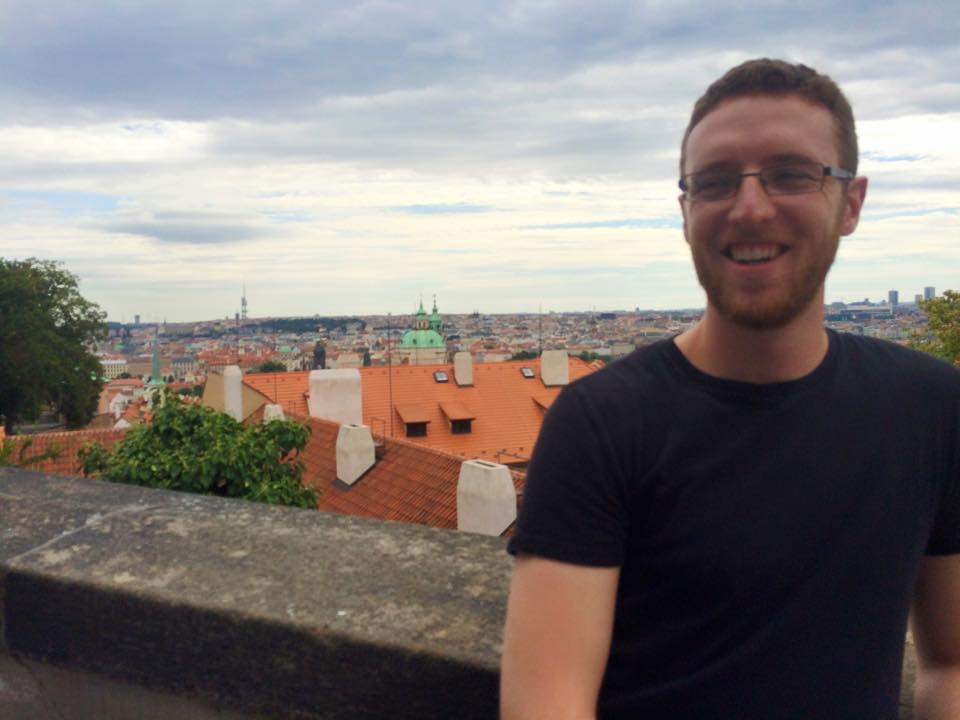
\includegraphics[width=1in,height=1.25in,clip,keepaspectratio]{pic/nick}}]{Nicholas Houghton}
	received his masters in Applied Science from the University of Victoria, BC, Canada in 2016.
	He received the B.Eng degree in Computer Engineering in 2015 also from the University of Victoria.
\end{IEEEbiography}
\vfill
\begin{IEEEbiography}[{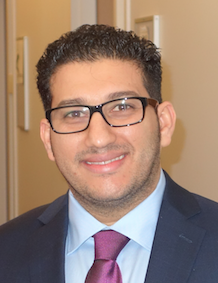
\includegraphics[width=1in,height=1.25in,clip,keepaspectratio]{pic/samer}}]{Samer Moein}
	received the Ph.D. degree in Computer Engineering from the University
	of Victoria, Victoria, BC, Canada, in 2015.
	Currently, he is a Post Doctoral Fellow in the Department of Electrical and Computer
	Engineering at the University of Victoria.
	He received the B.Sc. degree in Computer
	Engineering from Kuwait University, Kuwait in 2004, and the M.Sc.
	degree in Computer Engineering from Kuwait University, Kuwait in 2011.
	His research interests include computer security, cryptography, and crypto-processors.
\end{IEEEbiography}
\begin{IEEEbiography}[{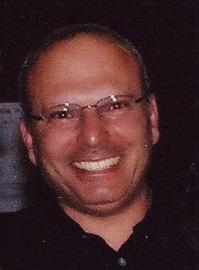
\includegraphics[width=1in,height=1.25in,clip,keepaspectratio]{pic/gebali}}]{Fayez Gebali}
	received the B.Sc. degree in Electrical Engineering (first class honors) from Cairo University,
	the B.Sc. degree in Mathematics (first class honors) from Ain Shams University,
	and the Ph.D. degree in Electrical Engineering form the University of British Columbia where he held an NSERC postgraduate scholarship.
	Dr. Gebali is a Professor in the Department of Electrical and Computer Engineering at the University of Victoria,
	and is currently Department Chair.
	His research interests include parallel algorithms, networks-on-chip, three-dimensional integrated circuits, digital communications, and computer arithmetic.
\end{IEEEbiography}
\vfill
% You can push biographies down or up by placing
% a \vfill before or after them. The appropriate
% use of \vfill depends on what kind of text is
% on the last page and whether or not the columns
% are being equalized.

%\vfill

% Can be used to pull up biographies so that the bottom of the last one
% is flush with the other column.
%\enlargethispage{-5in}



% that's all folks
\end{document}


